% Hamzeh Khanpour
% Ultra-cold muons for the LHC, AGH University of Krakow, 24--26 September 2026
% Talk: Two-Photon Physics
% Rebuilt from the original Ultra-cold-muons_2026_Slides_LHmuC LaTeX project.

\documentclass[aspectratio=1610,english]{beamer}

\usepackage{babel}
\usepackage[T1]{fontenc}
\usepackage[utf8]{inputenc}
\usepackage{lmodern}
\usepackage{amsmath,amssymb,bm}
\usepackage{booktabs}
\usepackage{graphicx}
\usepackage{array}
\usepackage{ragged2e}
\usepackage{etoolbox}
\usepackage{tikz}
\usepackage{comment}
\usepackage{tikz-feynman}
\tikzfeynmanset{compat=1.1.0}
\usetikzlibrary{calc,positioning,arrows.meta,decorations.pathmorphing,patterns,shapes.geometric,fit}
\usepackage{hyperref}
\usepackage[table]{xcolor}

\makeatletter
\patchcmd{\itemize}{\raggedright}{\justifying}{}{}
\patchcmd{\beamer@enum@}{\raggedright}{\justifying}{}{}
\patchcmd{\@@description}{\raggedright}{\justifying}{}{}
\makeatother

\mode<beamer>{
  \definecolor{links}{HTML}{2A1B81}
  \hypersetup{pdfpagemode=FullScreen,colorlinks,linkcolor=,urlcolor=links}
  \usetheme[parttitle=rightfooter]{AGH}
}

\graphicspath{{figures/}{./}}

\definecolor{LHRed}{RGB}{170,20,30}
\definecolor{LHBlue}{RGB}{25,60,180}
\definecolor{LHGreen}{RGB}{0,120,60}
\definecolor{LHOrange}{RGB}{210,110,20}
\definecolor{LHPurple}{RGB}{110,60,160}

\newcommand{\LHCmu}{LH$\mu$C}
\newcommand{\helplogo}{%
\begin{tikzpicture}[remember picture,overlay]
\node[anchor=north east,xshift=-0.10cm,yshift=-0.35cm] at (current page.north east)
{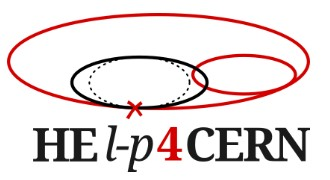
\includegraphics[width=1.5cm]{HELP4CERN.jpg}};
\end{tikzpicture}}

\newcommand{\sourceline}[1]{%
\vfill\hspace*{0.15cm}{\tiny\color{black!70}#1}\par}

\newcommand{\takehome}[1]{%
\begin{alertblock}{Take-home message}\small\justifying #1\end{alertblock}}

\newcommand{\placeholdergraphic}[2]{%
\begin{center}
\fbox{\parbox[c][#2][c]{0.92\linewidth}{\centering\vspace{1ex}\textbf{Figure placeholder}\\[0.6ex]\small #1\vspace{1ex}}}
\end{center}}

\title[Two-photon Physics at \LHCmu]{\justifying Two-Photon Physics at the LH$\mu$C}
\subtitle{High-energy $\gamma\gamma$ interactions in $\mu p$ collisions}
\author[Hamzeh Khanpour]{Hamzeh Khanpour\\{\scriptsize AGH University of Krakow}}
\institute[AGH]{\color{magenta}\textbf{(on behalf of HELP4CERN Study Group)}}
\date{{\setlength{\fboxsep}{4pt}\colorbox{cyan!15}{\strut Ultra-cold muons for the LHC, AGH Krakow, 24--26 September 2026}}}

\begin{document}

% --------------------------------------------------------------------------
% Slide 1 -- Adapted from original Ultra-cold-muons title slide
% --------------------------------------------------------------------------
\begin{frame}
\begin{tikzpicture}[remember picture,overlay]
\node[anchor=north east,xshift=-0.60cm,yshift=-1.50cm] at (current page.north east)
{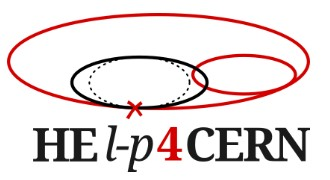
\includegraphics[width=2.5cm]{HELP4CERN.jpg}};
\end{tikzpicture}
\titlepage
\end{frame}

% --------------------------------------------------------------------------
% Slide 2 -- Photon-focused outline
% --------------------------------------------------------------------------
\begin{frame}{Outline}
\tableofcontents
\begin{tikzpicture}[remember picture,overlay]
\node[anchor=north east,xshift=-0.60cm,yshift=-1.50cm] at (current page.north east)
{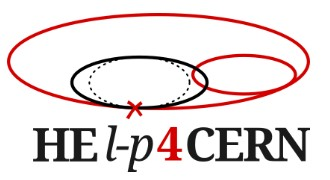
\includegraphics[width=2.5cm]{HELP4CERN.jpg}};
\end{tikzpicture}
\end{frame}

\section{LH$\mu$C and the $\gamma\gamma$ opportunity}

% --------------------------------------------------------------------------
% Slide 3 -- Adapted from original motivation slide
% Source: DIS2026 HET deck + yy_lhec introduction
% --------------------------------------------------------------------------
\begin{frame}{Why a muon-hadron collider for two-photon physics?}
\begin{itemize}
\item A muon-hadron collider combines a \textbf{clean lepton-hadron initial state} with a multi-TeV centre-of-mass energy.
\item Replacing the electron beam by a muon beam strongly relaxes the synchrotron-radiation limitation, making much higher lepton-beam energies possible.
\item The $\mu p$ environment remains experimentally cleaner than $pp$ for many exclusive and semi-exclusive final states: negligible pile-up is a central advantage of the lepton-hadron concept.
\item Both beams radiate photons. Their electromagnetic fields therefore create a high-energy $\gamma\gamma$ collider \emph{inside} the $\mu p$ machine.
\end{itemize}
\takehome{LH$\mu$C combines a high-energy photon source from the muon beam with the electromagnetic photon field of the proton, opening a distinctive high-energy $\gamma\gamma$ programme.}
\sourceline{Physics motivation adapted from the HELP4CERN / DIS2026 decks and the LHeC $\gamma\gamma$ study.}
\helplogo
\end{frame}

% --------------------------------------------------------------------------
% Slide 4 -- Adapted from original benchmark working-points slide
% --------------------------------------------------------------------------
\begin{frame}{LH$\mu$C@CERN: benchmark working points}
\begin{columns}[T]
\begin{column}{0.61\textwidth}
\begin{itemize}\small
\item \textbf{Workshop focus:} $E_\mu=500~\mathrm{GeV}$ and $E_p=7~\mathrm{TeV}$,
\[
\sqrt{s_{\mu p}}\simeq 3.7~\mathrm{TeV},\qquad \mathcal L_{\rm int}\simeq 250~\mathrm{fb}^{-1}.
\]
\item Higher-energy HELP4CERN working points remain useful for scaling studies:
\begin{itemize}\small
\item $E_\mu=1~\mathrm{TeV}\Rightarrow\sqrt{s}\simeq5.3~\mathrm{TeV}$,
\item $E_\mu=2~\mathrm{TeV}\Rightarrow\sqrt{s}\simeq7.5~\mathrm{TeV}$.
\end{itemize}
\item Already the 500 GeV option enters a qualitatively new $\gamma\gamma$ mass regime compared with LHeC.
\end{itemize}
\begin{block}{This talk}
\small The quantitative $\gamma\gamma$ benchmarks shown below emphasise the 500 GeV $\mu$ beam whenever dedicated results exist.
\end{block}
\end{column}
\begin{column}{0.36\textwidth}
\begin{alertblock}{Working points}\small
\begin{tabular}{@{}lll@{}}
\toprule
 & $E_\ell$ & $\sqrt{s}$\\
\midrule
LHeC & 50 GeV & 1.2 TeV\\
LH$\mu$C & \textbf{500 GeV} & \textbf{3.7 TeV}\\
LH$\mu$C & 1 TeV & 5.3 TeV\\
LH$\mu$C & 2 TeV & 7.5 TeV\\
\bottomrule
\end{tabular}
\end{alertblock}
\centering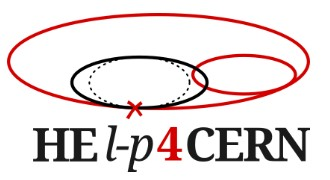
\includegraphics[width=0.42\linewidth]{HELP4CERN.jpg}
\end{column}
\end{columns}
\sourceline{HELP4CERN benchmark set used in the DIS2026 HET study.}
\end{frame}

% --------------------------------------------------------------------------
% Slide 5 -- New conceptual transition slide
% --------------------------------------------------------------------------

\begin{frame}{A high-energy $\gamma\gamma$ collider inside $\mu p$ collisions}
\begin{columns}[T]
\begin{column}{0.57\textwidth}
\centering
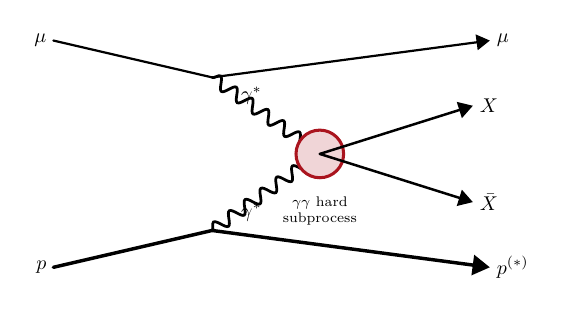
\begin{tikzpicture}[scale=0.72,transform shape,>=Triangle,line cap=round]
\coordinate (mi) at (-4,2); \coordinate (mv) at (-1.2,1.35); \coordinate (mo) at (3.7,2);
\coordinate (pi) at (-4,-2); \coordinate (pv) at (-1.2,-1.35); \coordinate (po) at (3.7,-2);
\coordinate (c) at (0.7,0);
\draw[->,line width=0.8pt] (mi)--(mv)--(mo);
\draw[->,line width=1.25pt] (pi)--(pv)--(po);
\draw[decorate,decoration={snake,amplitude=2.2pt,segment length=7pt},line width=1pt] (mv)--(c);
\draw[decorate,decoration={snake,amplitude=2.2pt,segment length=7pt},line width=1pt] (pv)--(c);
\draw[fill=LHRed!18,draw=LHRed,line width=1.1pt] (c) circle (0.42);
\draw[->,line width=0.9pt] (c)--(3.4,0.85); \draw[->,line width=0.9pt] (c)--(3.4,-0.85);
\node[left] at (mi) {$\mu$}; \node[right] at (mo) {$\mu$};
\node[left] at (pi) {$p$}; \node[right] at (po) {$p^{(*)}$};
\node[above left] at (-0.2,0.75) {$\gamma^*$}; \node[below left] at (-0.2,-0.75) {$\gamma^*$};
\node[right] at (3.4,0.85) {$X$}; \node[right] at (3.4,-0.85) {$\bar X$};
\node[font=\scriptsize,align=center] at (0.7,-1.0) {$\gamma\gamma$ hard\\subprocess};
\end{tikzpicture}
\vspace{0.2em}
{\scriptsize Both beams act as photon sources; the central system is produced by $\gamma\gamma$ fusion.}
\end{column}
\begin{column}{0.40\textwidth}
\begin{block}{Factorised picture}\scriptsize
\[
\mu\to\mu+\gamma^*,\qquad p\to p^{(*)}+\gamma^*,
\]
\[
\gamma\gamma\to X,\qquad \mu p\to\mu+X+p^{(*)}.
\]
\end{block}
\begin{itemize}\scriptsize
\item \textcolor{LHGreen}{Elastic}: proton remains intact.
\item \textcolor{LHOrange}{Tagged elastic}: intact proton measured near the beam.
\item \textcolor{LHRed}{Dissociative}: proton breaks into a system of mass $M_N$.
\end{itemize}
\begin{alertblock}{Key point}\scriptsize
One parent $\mu p$ data set contains several distinct $\gamma\gamma$ topologies with different photon virtualities and experimental handles.
\end{alertblock}
\end{column}
\end{columns}
\helplogo
\end{frame}

% --------------------------------------------------------------------------
% Slide 6 -- New topology slide
% Source: yy_lhec, Fig. 3 logic and EPA section
% --------------------------------------------------------------------------
\begin{frame}{Two-photon production topologies: elastic, tagged and proton-dissociative}
\begin{columns}[T]
\begin{column}{0.48\textwidth}
\centering
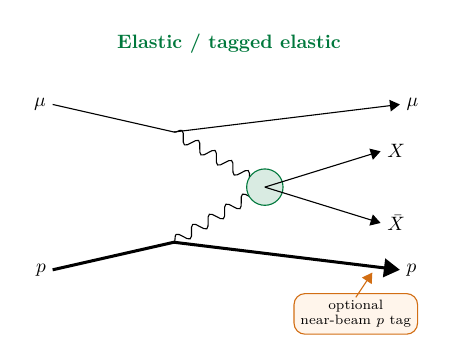
\begin{tikzpicture}[scale=0.70,transform shape,>=Triangle]
\node[font=\bfseries\color{LHGreen}] at (0,2.6) {Elastic / tagged elastic};
\coordinate (mi) at (-3.2,1.5);\coordinate (mv) at (-1.0,1.0);\coordinate (mo) at (3.1,1.5);
\coordinate (pi) at (-3.2,-1.5);\coordinate (pv) at (-1.0,-1.0);\coordinate (po) at (3.1,-1.5);
\coordinate (c) at (0.65,0);
\draw[->] (mi)--(mv)--(mo);\draw[->,line width=1.1pt] (pi)--(pv)--(po);
\draw[decorate,decoration={snake,amplitude=2pt,segment length=7pt}] (mv)--(c);
\draw[decorate,decoration={snake,amplitude=2pt,segment length=7pt}] (pv)--(c);
\draw[fill=LHGreen!15,draw=LHGreen] (c) circle (0.33);
\draw[->] (c)--(2.75,0.65);\draw[->] (c)--(2.75,-0.65);
\node[left] at (mi) {$\mu$};\node[right] at (mo) {$\mu$};\node[left] at (pi) {$p$};\node[right] at (po) {$p$};
\node[right] at (2.75,0.65) {$X$};\node[right] at (2.75,-0.65) {$\bar X$};
\node[draw=LHOrange,rounded corners,fill=orange!8,font=\scriptsize,align=center] at (2.3,-2.3) {optional\\near-beam $p$ tag};
\draw[->,LHOrange] (2.3,-2.0)--(2.6,-1.55);
\end{tikzpicture}
\begin{itemize}\scriptsize
\item Proton electromagnetic form factors control the elastic flux.
\item A near-beam tag can over-constrain event kinematics.
\end{itemize}
\end{column}
\begin{column}{0.48\textwidth}
\centering
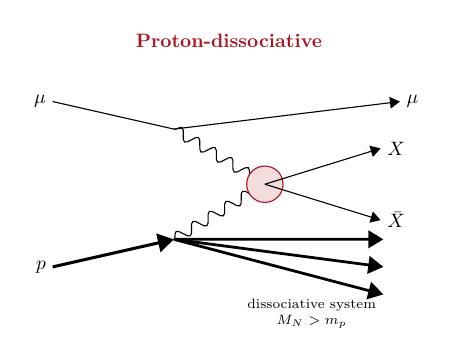
\begin{tikzpicture}[scale=0.70,transform shape,>=Triangle]
\node[font=\bfseries\color{LHRed}] at (0,2.6) {Proton-dissociative};
\coordinate (mi) at (-3.2,1.5);\coordinate (mv) at (-1.0,1.0);\coordinate (mo) at (3.1,1.5);
\coordinate (pi) at (-3.2,-1.5);\coordinate (pv) at (-1.0,-1.0);\coordinate (c) at (0.65,0);
\draw[->] (mi)--(mv)--(mo);\draw[->,line width=1.1pt] (pi)--(pv);
\draw[decorate,decoration={snake,amplitude=2pt,segment length=7pt}] (mv)--(c);
\draw[decorate,decoration={snake,amplitude=2pt,segment length=7pt}] (pv)--(c);
\draw[fill=LHRed!15,draw=LHRed] (c) circle (0.33);
\draw[->] (c)--(2.75,0.65);\draw[->] (c)--(2.75,-0.65);
\draw[->,line width=1.0pt] (pv)--(2.8,-1.0);\draw[->,line width=1.0pt] (pv)--(2.8,-1.5);\draw[->,line width=1.0pt] (pv)--(2.8,-2.0);
\node[left] at (mi) {$\mu$};\node[right] at (mo) {$\mu$};\node[left] at (pi) {$p$};
\node[right] at (2.75,0.65) {$X$};\node[right] at (2.75,-0.65) {$\bar X$};
\node[font=\scriptsize,align=center] at (1.5,-2.35) {dissociative system\\$M_N>m_p$};
\end{tikzpicture}
\begin{itemize}\scriptsize
\item Inelastic flux is described through proton structure functions.
\item Larger $M_N$ and $Q_p^2$ increase the accessible luminosity but also modelling dependence.
\end{itemize}
\end{column}
\end{columns}
\sourceline{Topology definitions follow the LHeC $\gamma\gamma$ study; the same classification carries directly to $\mu p$.}
\helplogo
\end{frame}

\section{Equivalent Photon Approximation and $\gamma\gamma$ luminosity}

% --------------------------------------------------------------------------
% Slide 7 -- Source: yy_lhec EPA section
% --------------------------------------------------------------------------

\begin{frame}{Equivalent Photon Approximation: factorising the $\mu p$ cross section}
\begin{block}{EPA master relation}\small
\[
\boxed{\displaystyle
\sigma_{\mu p}=\int dy_\mu\,dy_p\;\Phi_\mu(y_\mu)\Phi_p(y_p)\,\sigma_{\gamma\gamma}(W)
      =\int dW\;S_{\gamma\gamma}(W)\,\sigma_{\gamma\gamma}(W)}
\]
\end{block}
\begin{columns}[T]
\begin{column}{0.55\textwidth}
\begin{itemize}\small
\item $\Phi_\mu$ and $\Phi_p$ are the equivalent-photon fluxes radiated by the two beams.
\item The hard subprocess $\gamma\gamma\to X$ factorises from photon emission, in close analogy with partonic convolutions.
\item $S_{\gamma\gamma}(W)$ packages the two fluxes into the effective two-photon luminosity spectrum.
\end{itemize}
\end{column}
\begin{column}{0.41\textwidth}
\begin{alertblock}{Kinematic variables}\small
\[
y_\mu=\frac{E_\gamma^{(\mu)}}{E_\mu},\qquad
 y_p=\frac{E_\gamma^{(p)}}{E_p},
\]
\[
W\equiv W_{\gamma\gamma}.
\]
\end{alertblock}
\end{column}
\end{columns}
\sourceline{EPA formalism: yy\_lhec / draft\_yy\_lhec.}
\helplogo
\end{frame}

% --------------------------------------------------------------------------
% Slide 8 -- Source: yy_lhec theory input
% --------------------------------------------------------------------------

\begin{frame}{Equivalent photon fluxes from the muon and proton}
\begin{columns}[T]
\begin{column}{0.60\textwidth}
\begin{block}{Generic EPA flux}\scriptsize
\[
\resizebox{0.96\linewidth}{!}{$\displaystyle
\Phi_\gamma(y)=\frac{\alpha}{\pi y}\int\frac{dQ^2}{Q^2}
\left[(1-y)\left(1-\frac{Q^2_{\min}}{Q^2}\right)F_E(Q^2)
+\frac{y^2}{2}F_M(Q^2)\right]$}
\]
\[
Q^2_{\min}=\frac{M^2y^2}{1-y}.
\]
\end{block}
\begin{itemize}\scriptsize
\item Point-like lepton: $F_E=F_M=1$ and $M=m_\mu$.
\item The muon mass raises $Q^2_{\min}$ relative to an electron at the same photon energy fraction $y$.
\end{itemize}
\end{column}
\begin{column}{0.36\textwidth}
\begin{alertblock}{Elastic proton emission}\scriptsize
\[
F_M=G_M^2,
\]
\[
F_E=\frac{4m_p^2G_E^2+Q^2G_M^2}{4m_p^2+Q^2}.
\]
The dipole form factors suppress large $Q_p^2$.
\end{alertblock}
\begin{block}{Proton dissociation}\scriptsize
For $p\to X$, structure functions replace elastic form factors and the flux depends on the dissociative mass $M_N$.
\end{block}
\end{column}
\end{columns}
\sourceline{Photon-flux formula and proton form factors: theory input of yy\_lhec / draft\_yy\_lhec.}
\helplogo
\end{frame}

% --------------------------------------------------------------------------
% Slide 9 -- Adapted from current deck Syy plot
% --------------------------------------------------------------------------

\begin{frame}{The $\gamma\gamma$ luminosity spectrum $S_{\gamma\gamma}(W)$}
\begin{columns}[T]
\begin{column}{0.57\textwidth}
\centering
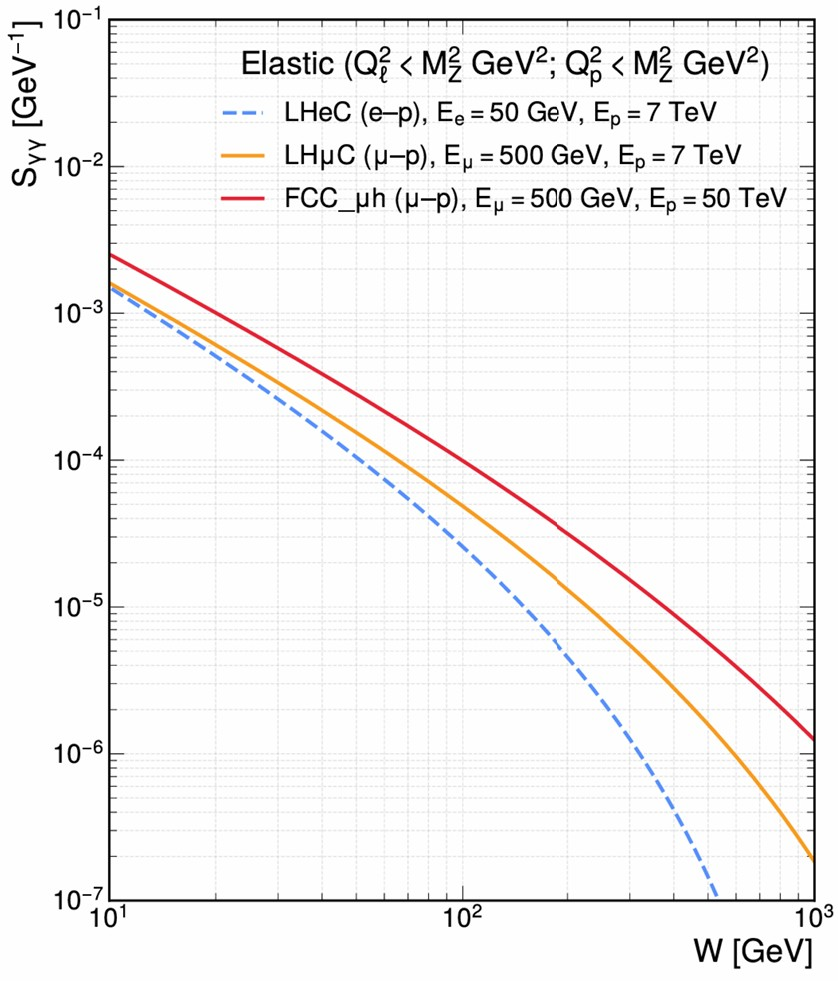
\includegraphics[width=0.78\linewidth]{Syy.jpg}
\end{column}
\begin{column}{0.40\textwidth}
\begin{block}{$S_{\gamma\gamma}$ tells us}\scriptsize
The fraction of the parent lepton--proton luminosity available for two-photon collisions at invariant mass $W$.
\end{block}
\begin{itemize}\scriptsize
\item The \textcolor{LHOrange}{500 GeV LH$\mu$C} spectrum extends well beyond the LHeC reach.
\item A harder spectrum benefits the $WW$, $ZZ$, $t\bar t$ and charged-BSM thresholds.
\item Energy-growing EFT effects are naturally amplified in the high-$W$ tail.
\end{itemize}
\vspace{0.2em}
{\scriptsize\color{LHRed}\textbf{LH$\mu$C message:} the gain is not only in total statistics; the $\gamma\gamma$ spectrum is substantially harder.}
\end{column}
\end{columns}
\sourceline{Existing HELP4CERN elastic-luminosity comparison; orange: $E_\mu=500$ GeV, $E_p=7$ TeV.}
\helplogo
\end{frame}

% --------------------------------------------------------------------------
% Slide 10 -- Source: yy_lhec Fig. 2; LHeC reference topology study
% --------------------------------------------------------------------------

\begin{frame}{Elastic vs. inelastic $\gamma\gamma$ luminosity and forward proton tagging}
\begin{columns}[T]
\begin{column}{0.64\textwidth}
\centering
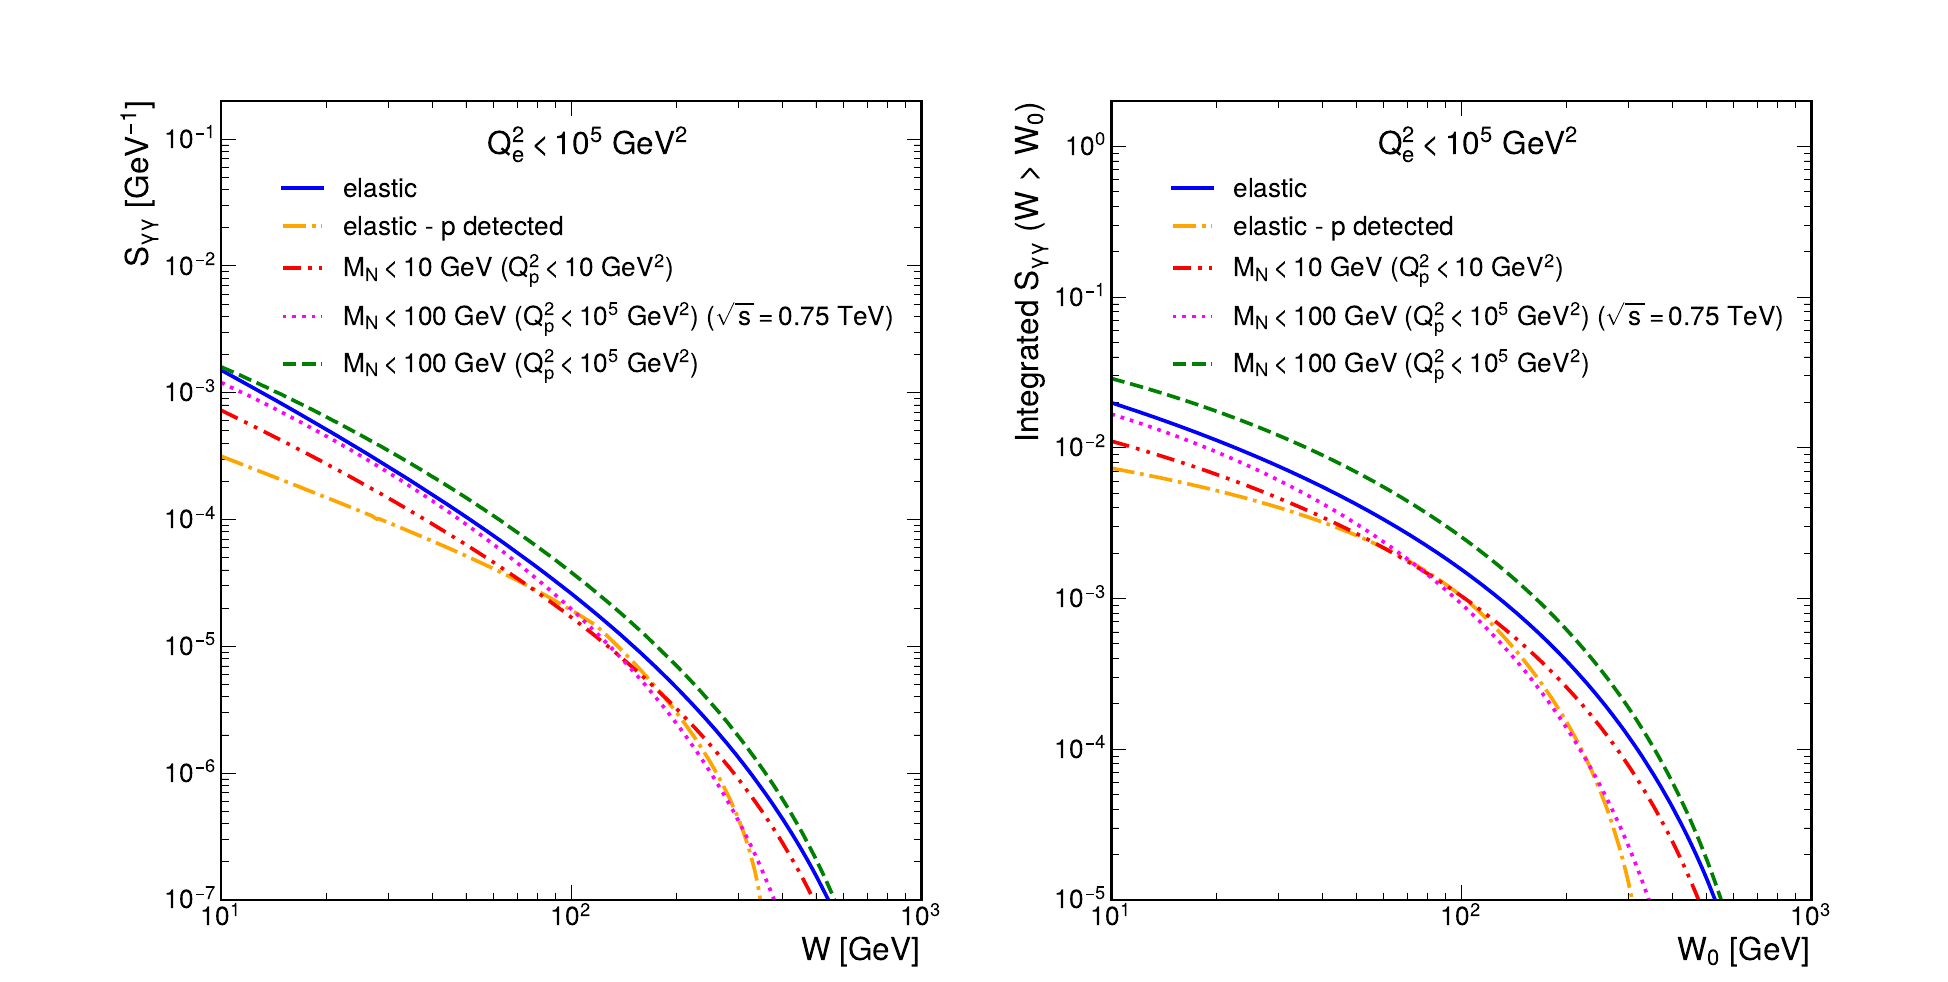
\includegraphics[width=0.86\linewidth]{luminosity_elastic_inelastic.png}
\end{column}
\begin{column}{0.33\textwidth}
\begin{alertblock}{LHeC reference study}\tiny
The detailed calculation separates elastic, tagged elastic ($0.01<y_p<0.1$), and proton-dissociative photon emission for several $M_N$ and $Q_p^2$ ranges.
\end{alertblock}
\begin{itemize}\scriptsize
\item Larger allowed dissociative masses increase the usable $\gamma\gamma$ luminosity.
\item A forward proton tag improves kinematic closure, especially for final states with neutrinos.
\item Low pile-up means proton tagging need not be mandatory for every clean channel.
\end{itemize}
\end{column}
\end{columns}
\sourceline{LHeC $\gamma\gamma$ paper: luminosity spectrum and near-beam tagging discussion; topology logic transfers to LH$\mu$C.}
\helplogo
\end{frame}

% --------------------------------------------------------------------------
% Slide 11 -- Source: draft_yy_lhec appendices C/D
% --------------------------------------------------------------------------

\begin{frame}{Beyond the simplest EPA: photon virtuality and exact $W_{\gamma\gamma}$ kinematics}
\begin{columns}[T]
\begin{column}{0.50\textwidth}
\begin{block}{High-energy approximation}\small
\[
W^2\simeq y_\ell y_p s.
\]
\end{block}
\begin{alertblock}{Exact elastic relation in the updated study}\small
\[
\boxed{W^2=-Q_\ell^2+y_\ell y_p s}
\]
{\scriptsize The paper writes $\ell=e$; the same lepton-side kinematics applies after $e\to\mu$.}
\end{alertblock}
\end{column}
\begin{column}{0.46\textwidth}
\begin{itemize}\scriptsize
\item The approximation is excellent when photon virtualities are negligible relative to $W^2$.
\item For proton dissociation, the exact expression also depends on $Q_p^2$ and $M_N$.
\item Elastic EPA agrees at percent level with matrix-element generators once the proper $W$ definition is used; inelastic modelling is more sensitive to the dissociative phase space.
\end{itemize}
\begin{block}{Precision lesson}\scriptsize
At sizeable $Q^2$, correct $W_{\gamma\gamma}$ reconstruction is part of the physics model, not a cosmetic refinement.
\end{block}
\end{column}
\end{columns}
\sourceline{Updated exact-kinematics study: draft\_yy\_lhec, Appendices C--E.}
\helplogo
\end{frame}

% --------------------------------------------------------------------------
\section{Standard-Model $\gamma\gamma$ processes}

% Slide 12 -- New bridge from luminosity to subprocesses
% --------------------------------------------------------------------------
\begin{frame}{From photon luminosity to physics: $\gamma\gamma\to X$}
\begin{block}{Collider rate}
\[
\sigma\!\left(\mu p\to\mu\,X\,p^{(*)}\right)
= S_{\gamma\gamma}\otimes\sigma(\gamma\gamma\to X).
\]
\end{block}
\vspace{0.2em}
\begin{center}
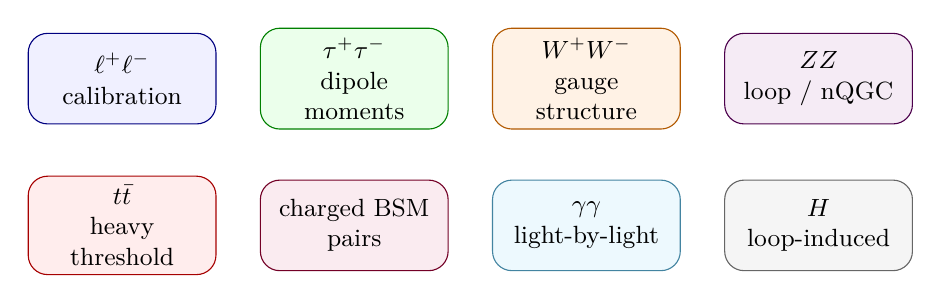
\begin{tikzpicture}[node distance=0.65cm and 0.55cm]
\tikzset{pbox/.style={rounded corners=7pt,draw=blue!50!black,fill=blue!6,minimum height=1.15cm,text width=2.15cm,align=center,font=\small}}
\node[pbox] (ll) {$\ell^+\ell^-$\\calibration};
\node[pbox,right=of ll,draw=green!50!black,fill=green!8] (ttau) {$\tau^+\tau^-$\\dipole moments};
\node[pbox,right=of ttau,draw=orange!70!black,fill=orange!10] (ww) {$W^+W^-$\\gauge structure};
\node[pbox,right=of ww,draw=violet!60!black,fill=violet!8] (zz) {$ZZ$\\loop / nQGC};
\node[pbox,below=of ll,draw=red!65!black,fill=red!7] (top) {$t\bar t$\\heavy threshold};
\node[pbox,right=of top,draw=purple!60!black,fill=purple!8] (bsm) {charged BSM\\pairs};
\node[pbox,right=of bsm,draw=cyan!60!black,fill=cyan!7] (lbl) {$\gamma\gamma$\\light-by-light};
\node[pbox,right=of lbl,draw=black!60,fill=black!4] (h) {$H$\\loop-induced};
\end{tikzpicture}
\end{center}
\takehome{The same photon luminosity supports precision QED, electroweak and loop physics, heavy thresholds, and direct searches for charged new states.}
\helplogo
\end{frame}

% --------------------------------------------------------------------------
% Slide 13 -- Adapted from existing exclusive gamma-gamma summary concept
% --------------------------------------------------------------------------

\begin{frame}{The high-energy $\gamma\gamma$ physics landscape at LH$\mu$C}
\begin{columns}[T]
\begin{column}{0.57\textwidth}
\centering
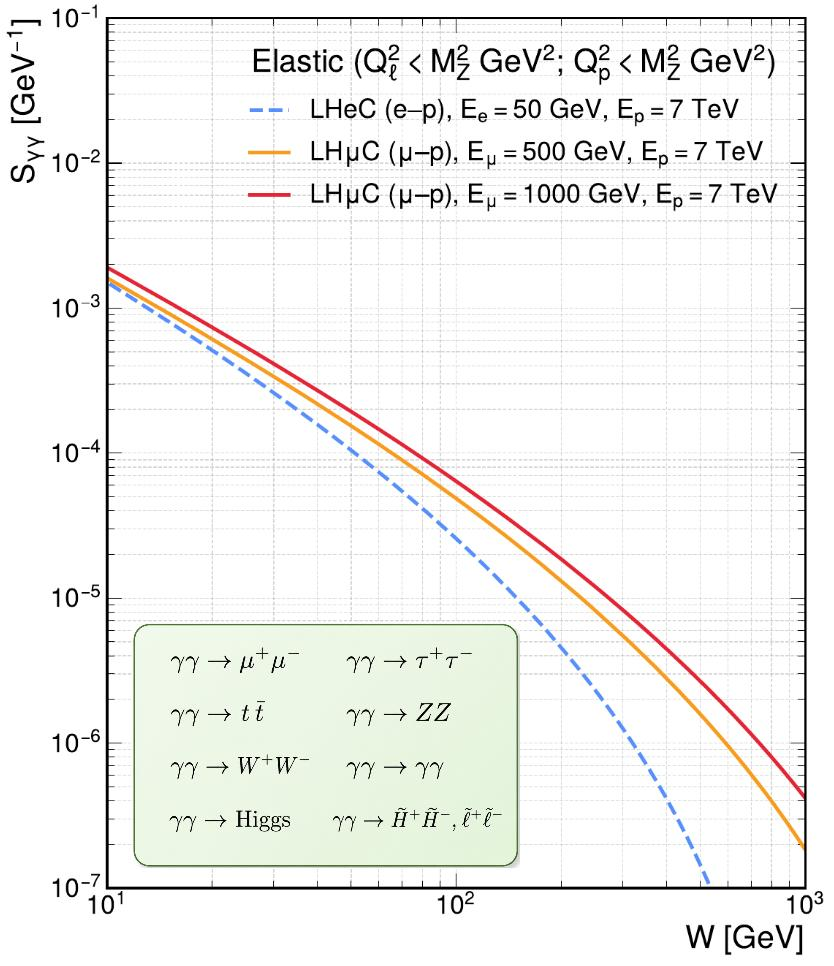
\includegraphics[width=0.82\linewidth]{Sgg_New.jpg}
\end{column}
\begin{column}{0.40\textwidth}
\begin{itemize}\scriptsize
\item \textcolor{LHGreen}{$\ell\ell,\tau\tau$}: high-rate QED calibration and dipole probes.
\item \textcolor{LHOrange}{$WW$}: sizeable SM rate and direct $\gamma\gamma WW$ coupling.
\item \textcolor{LHPurple}{$ZZ$}: loop-induced SM benchmark and neutral quartic couplings.
\item \textcolor{LHRed}{$t\bar t$}: heavy threshold and top electromagnetic structure.
\item \textcolor{LHBlue}{Charged BSM pairs}: production controlled mainly by electric charge and mass.
\item $\gamma\gamma$ and $H$: loop-induced quantum processes and complementary searches.
\end{itemize}
\end{column}
\end{columns}
\sourceline{Existing HELP4CERN threshold summary, adapted to the dedicated two-photon narrative.}
\helplogo
\end{frame}

% --------------------------------------------------------------------------
% Slide 14 -- Source: yy_lhec muon/electron-pair section
% --------------------------------------------------------------------------

\begin{frame}{$\gamma\gamma\to\ell^+\ell^-$: a standard candle for two-photon physics}
\begin{columns}[T]
\begin{column}{0.53\textwidth}
\begin{itemize}\scriptsize
\item $e^+e^-$ and $\mu^+\mu^-$ provide clean control samples for the complete $\gamma\gamma$ programme.
\item They test EPA modelling, acoplanarity and elastic/inelastic separation.
\item At LHeC, elastic EPA predictions agree with GRAPE and CepGen/LPAIR at the percent level for matched cuts and exact $W$ kinematics.
\end{itemize}
\begin{alertblock}{Elastic $\mu^+\mu^-$ benchmark at LHeC}\tiny
\centering
$Q^2_{e,p}<10~\mathrm{GeV}^2$\par\smallskip
\begin{tabular}{lcc}
\toprule
 & $W_0=10$ GeV & $W_0=100$ GeV\\
\midrule
EPA & 120.12 pb & 0.193 pb\\
CepGen/LPAIR & 118.31 pb & 0.191 pb\\
GRAPE (BH) & 121.37 pb & 0.193 pb\\
\bottomrule
\end{tabular}
\end{alertblock}
\end{column}
\begin{column}{0.43\textwidth}
\centering
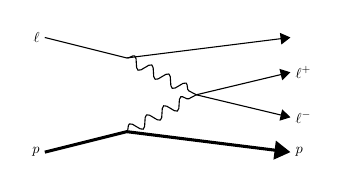
\begin{tikzpicture}[scale=0.52,transform shape,>=Triangle]
\coordinate (li) at (-3,1.4);\coordinate (lv) at (-1,0.9);\coordinate (lo) at (3,1.4);
\coordinate (pi) at (-3,-1.4);\coordinate (pv) at (-1,-0.9);\coordinate (po) at (3,-1.4);\coordinate (c) at (0.7,0);
\draw[->] (li)--(lv)--(lo);\draw[->,line width=1.1pt] (pi)--(pv)--(po);
\draw[decorate,decoration={snake,amplitude=2pt,segment length=7pt}] (lv)--(c);
\draw[decorate,decoration={snake,amplitude=2pt,segment length=7pt}] (pv)--(c);
\draw[->] (c)--(3,0.55);\draw[->] (c)--(3,-0.55);
\node[right] at (3,0.55) {$\ell^+$};\node[right] at (3,-0.55) {$\ell^-$};
\node[left] at (li) {$\ell$};\node[left] at (pi) {$p$};\node[right] at (po) {$p$};
\end{tikzpicture}
\begin{block}{Why it matters for LH$\mu$C}\scriptsize
The same QED process becomes a high-statistics calibration candle for the harder $\mu p$ photon spectrum and any forward-tagging strategy.
\end{block}
\end{column}
\end{columns}
\sourceline{LHeC $\gamma\gamma$ paper, Table 1 and calibration-candle discussion.}
\helplogo
\end{frame}

% --------------------------------------------------------------------------
% Slide 15 -- Adapted from existing tau cross-section slide
% --------------------------------------------------------------------------

\begin{frame}{$\gamma\gamma\to\tau^+\tau^-$: a high-statistics tau factory}
\begin{columns}[T]
\begin{column}{0.61\textwidth}
\centering
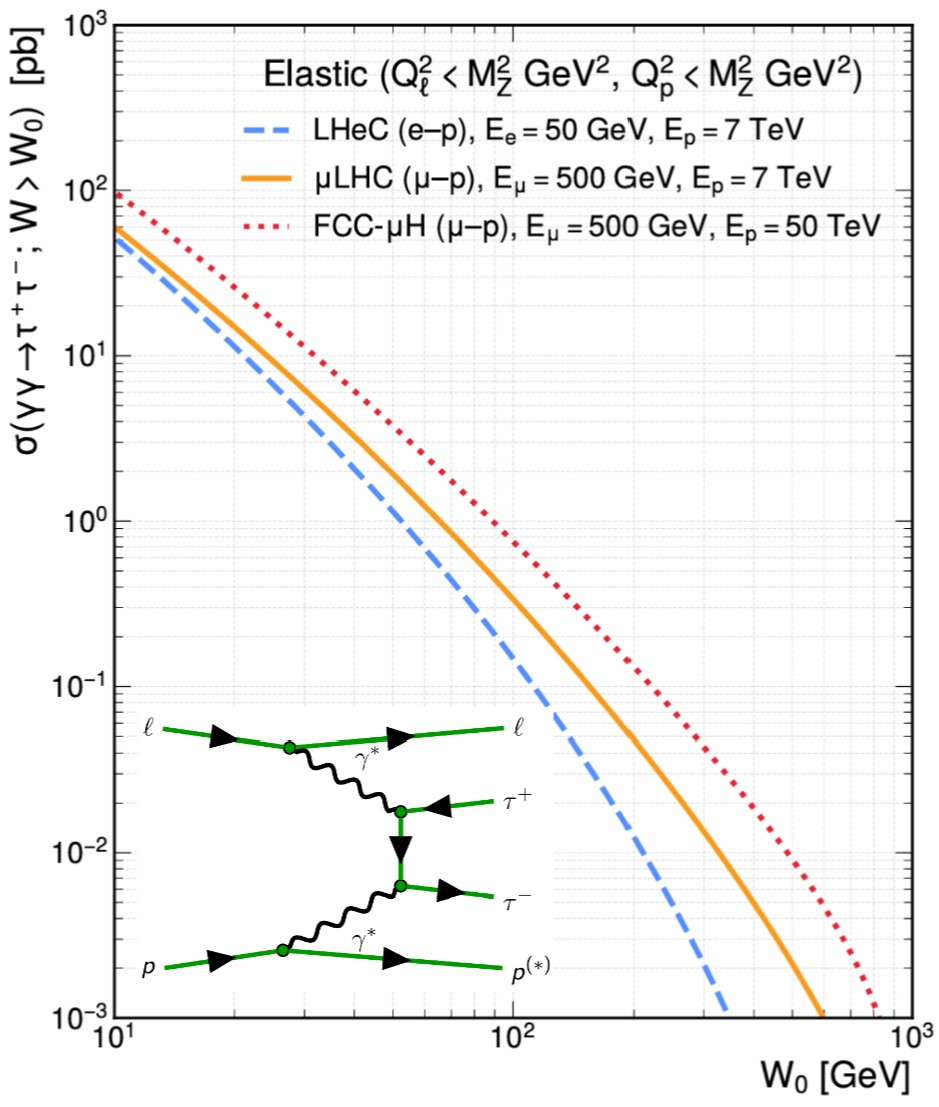
\includegraphics[width=0.82\linewidth]{elastic_tau_tau.jpg}
\end{column}
\begin{column}{0.35\textwidth}
\begin{alertblock}{Elastic benchmark}\scriptsize
\[
\sigma_{\rm el}^{\rm LHeC}\simeq 50.37~\mathrm{pb}
\]
\[
\boxed{\sigma_{\rm el}^{\rm LH\mu C(3.7)}\simeq 58.56~\mathrm{pb}}
\]
\end{alertblock}
\begin{itemize}\scriptsize
\item Large statistics make $\tau\tau$ a natural precision channel.
\item LH$\mu$C extends the accessible $M_{\tau\tau}$ tail.
\item The hard tail enhances sensitivity to non-standard $\gamma\tau\tau$ interactions.
\end{itemize}
\end{column}
\end{columns}
\sourceline{Elastic cross sections from the existing HELP4CERN two-photon calculations.}
\helplogo
\end{frame}

% --------------------------------------------------------------------------
\section{Precision / EFT probes: $\tau$ moments and gauge couplings}

% Slide 16 -- Source: dedicated tau-moments deck
% --------------------------------------------------------------------------

\begin{frame}{Anomalous $\tau$ electromagnetic moments: the $\gamma\tau\tau$ vertex}
\begin{columns}[T]
\begin{column}{0.60\textwidth}
\begin{block}{General electromagnetic vertex}\scriptsize
\[
\Gamma^\mu(q^2)=\gamma^\mu F_1(q^2)
+\frac{i\sigma^{\mu\nu}q_\nu}{2m_\tau}F_2(q^2)
+\sigma^{\mu\nu}q_\nu\gamma_5 F_3(q^2),
\]
\[
F_2(0)=a_\tau,\qquad F_3(0)=-\frac{2m_\tau}{e}\,d_\tau.
\]
\end{block}
\begin{itemize}\scriptsize
\item $a_\tau$: CP-even anomalous magnetic dipole moment.
\item $d_\tau$: CP-odd electric dipole moment.
\item $\gamma\gamma\to\tau^+\tau^-$ probes the vertex directly.
\end{itemize}
\end{column}
\begin{column}{0.36\textwidth}
\begin{alertblock}{SMEFT interpretation}\tiny
Gauge-invariant tau dipoles:
\[
\resizebox{0.94\linewidth}{!}{$\displaystyle
\bar L_\tau\sigma^{\mu\nu}\tau_R H
\left(\frac{C_{\tau B}}{\Lambda^2}B_{\mu\nu}
+\frac{C_{\tau W}}{\Lambda^2}W_{\mu\nu}\right)+\mathrm{h.c.}$}
\]
Real and imaginary coefficient combinations map respectively to magnetic and electric dipole deformations after electroweak symmetry breaking.
\end{alertblock}
\end{column}
\end{columns}
\sourceline{Dedicated anomalous-$\tau$ study, April 2026; updated benchmark on the next slide.}
\helplogo
\end{frame}

% --------------------------------------------------------------------------
% Slide 17 -- Source: updated draft_yy_lhec tau analysis
% --------------------------------------------------------------------------

\begin{frame}{Probing $\tau$ dipole moments in the high-$M_{\tau\tau}$ tail}
\begin{columns}[T]
\begin{column}{0.59\textwidth}
\centering
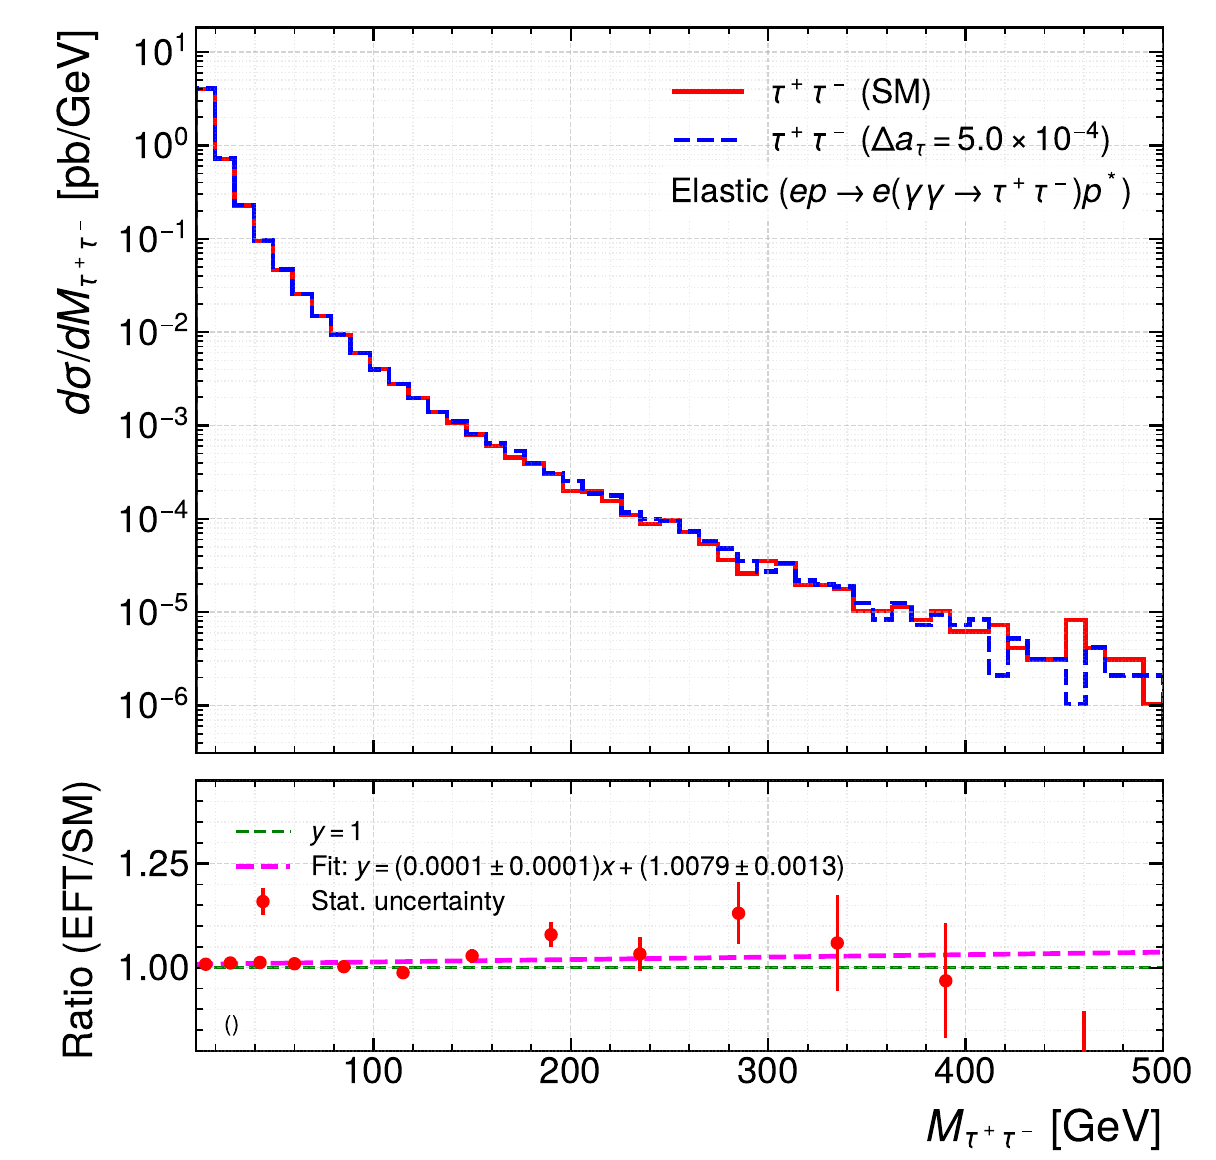
\includegraphics[width=0.76\linewidth]{tau_updated_Mtt.png}
\end{column}
\begin{column}{0.38\textwidth}
\begin{alertblock}{Updated paper benchmark}\scriptsize
The latest draft replaces the previous illustrative point by
\[
\boxed{\Delta a_\tau=5.0\times10^{-4}}.
\]
\end{alertblock}
\begin{itemize}\scriptsize
\item Shown: updated \textbf{LHeC elastic} reference calculation from the paper draft.
\item The EFT/SM ratio exposes the growing shape distortion in the hard $M_{\tau\tau}$ region.
\item The same SMEFT fit should be repeated for LH$\mu$C, whose harder spectrum gives more leverage at high mass.
\end{itemize}
\end{column}
\end{columns}
\sourceline{Updated draft\_yy\_lhec: $\Delta a_\tau=5\times10^{-4}$ and SMEFT translation.}
\helplogo
\end{frame}

% --------------------------------------------------------------------------
% Slide 18 -- Adapted from existing WW benchmark
% --------------------------------------------------------------------------

\begin{frame}{$\gamma\gamma\to W^+W^-$: a clean electroweak laboratory}
\begin{columns}[T]
\begin{column}{0.57\textwidth}
\centering
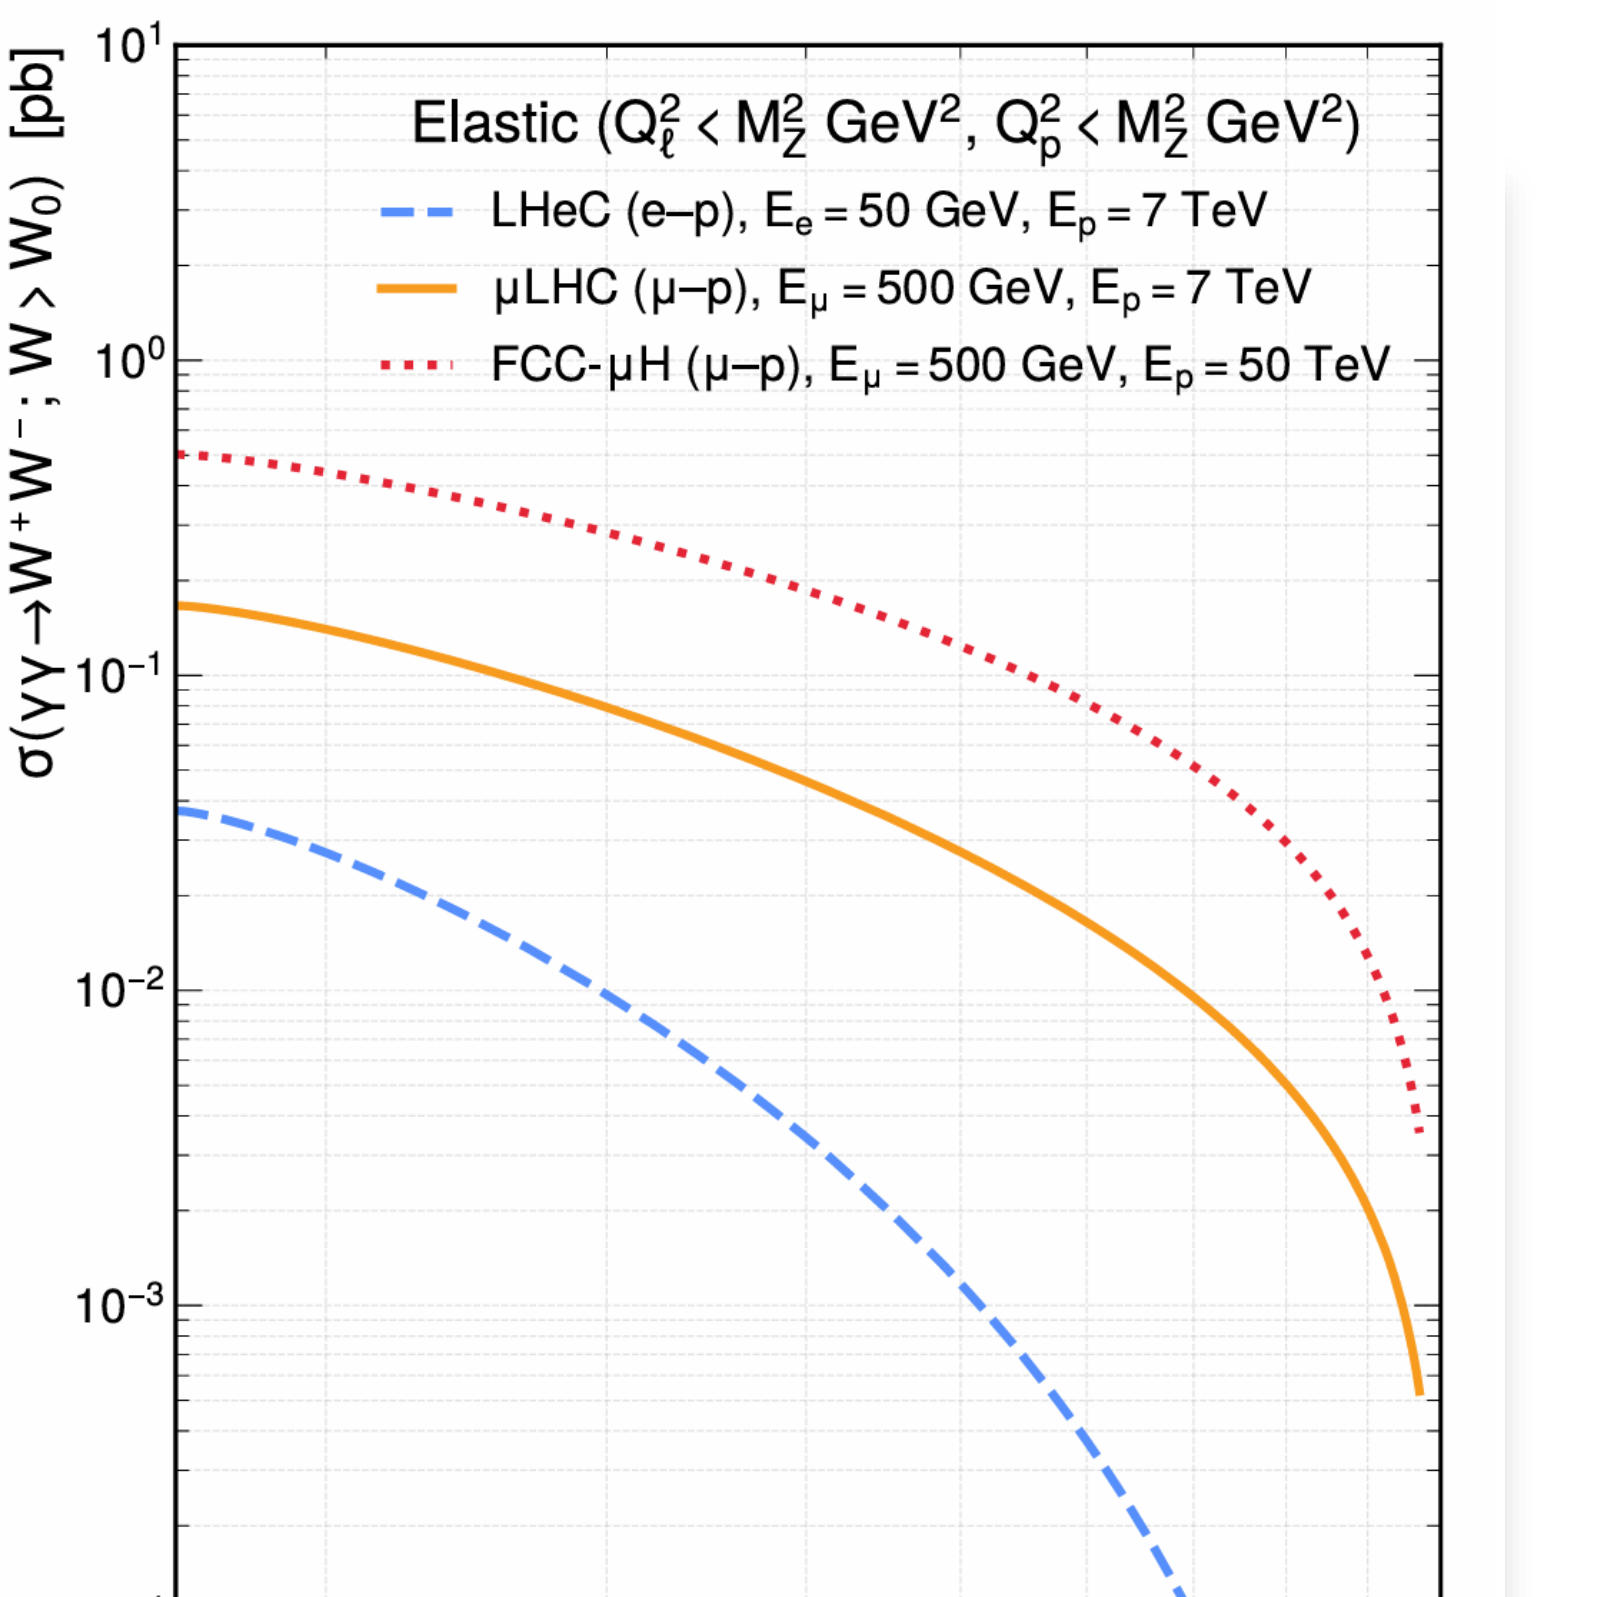
\includegraphics[width=0.68\linewidth]{ww_elastic_curve.png}
\end{column}
\begin{column}{0.39\textwidth}
\begin{alertblock}{Elastic rates}\scriptsize
\[
\sigma_{\rm el}^{\rm LHeC}\simeq0.037~\mathrm{pb}
\]
\[
\boxed{\sigma_{\rm el}^{\rm LH\mu C(3.7)}\simeq0.166~\mathrm{pb}}
\]
\end{alertblock}
\begin{itemize}\scriptsize
\item The $W$ threshold lies inside the high-luminosity $\gamma\gamma$ regime.
\item The process directly tests the SM $\gamma\gamma WW$ gauge structure.
\item The high-$M_{WW}$ tail is a clean lever arm for dimension-8 quartic-gauge operators.
\end{itemize}
\end{column}
\end{columns}
\sourceline{Existing HELP4CERN elastic $WW$ calculation; orange curve: LH$\mu$C@3.7 TeV.}
\helplogo
\end{frame}

% --------------------------------------------------------------------------
% Slide 19 -- Source: updated draft_yy_lhec WW aQGC analysis
% --------------------------------------------------------------------------

\begin{frame}{Anomalous quartic gauge couplings in $\gamma\gamma\to W^+W^-$}
\begin{columns}[T]
\begin{column}{0.59\textwidth}
\centering
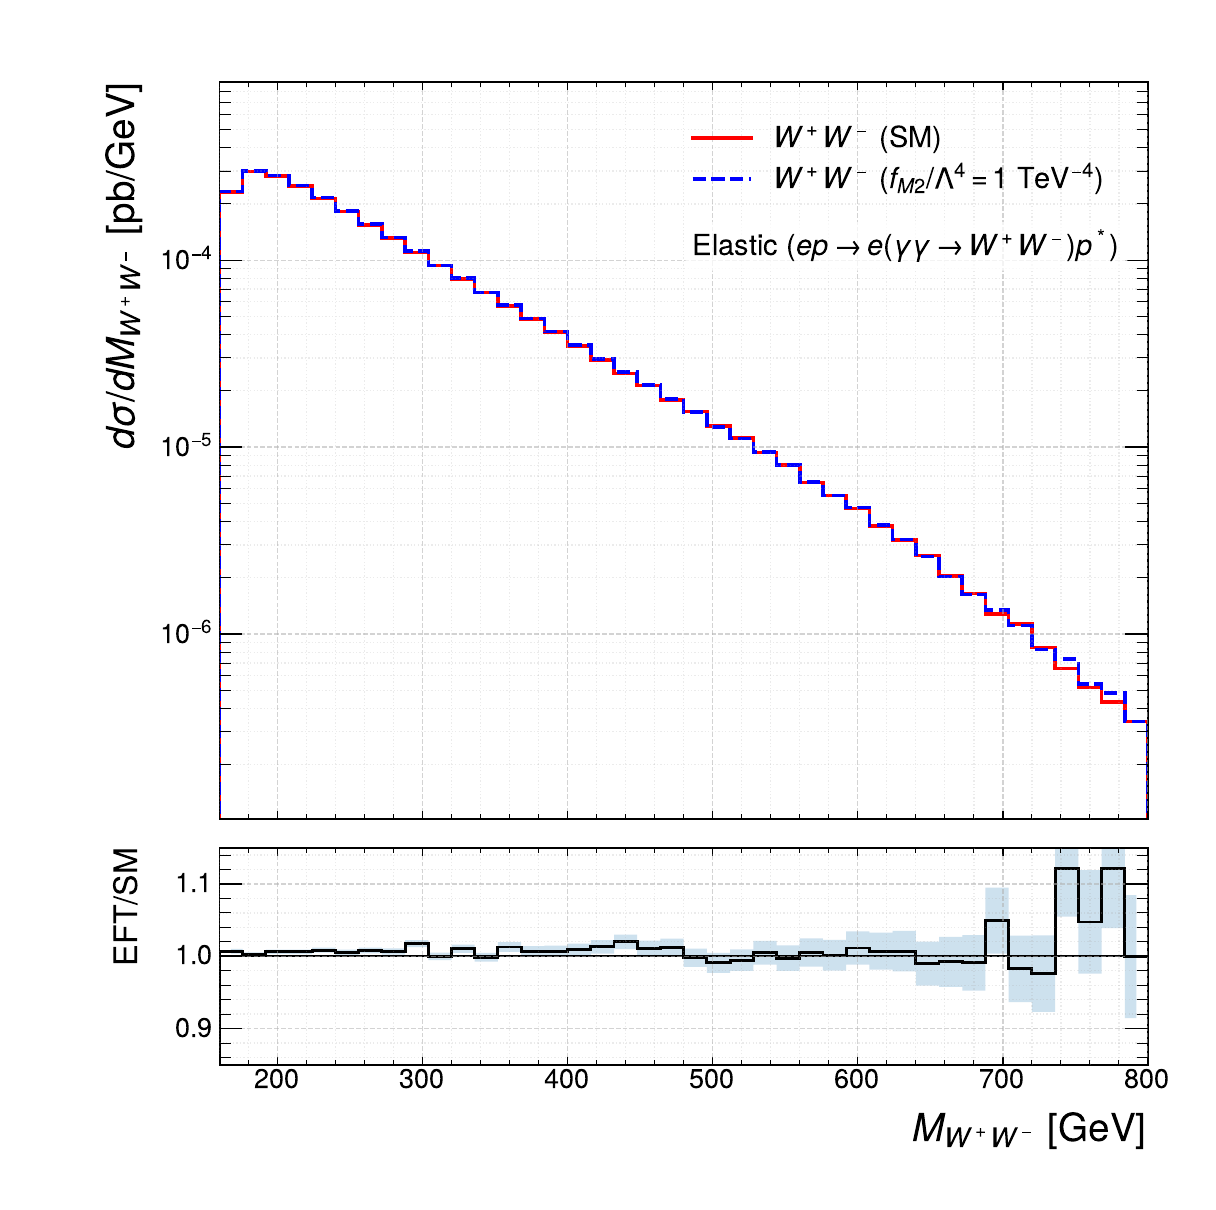
\includegraphics[width=0.73\linewidth]{ww_aqgc_updated.png}
\end{column}
\begin{column}{0.38\textwidth}
\begin{block}{Dimension-8 EFT}\scriptsize
\[
\mathcal L_{\rm eff}=\mathcal L_{\rm SM}+\sum_i\frac{f_i}{\Lambda^4}\mathcal O_i,
\]
\[
\frac{f_{M2}}{\Lambda^4}=1~\mathrm{TeV}^{-4}.
\]
\end{block}
\begin{itemize}\scriptsize
\item Shown: updated \textbf{LHeC elastic} reference from the draft.
\item EFT effects are tiny at low $M_{WW}$ and grow in the hard tail.
\item LH$\mu$C supplies the harder $W_{\gamma\gamma}$ spectrum needed to extend this strategy quantitatively.
\end{itemize}
\vspace{0.2em}
{\tiny\color{LHRed}\textbf{Scope:} no detector-level LH$\mu$C exclusion is claimed here; this is a defined next HELP4CERN study.}
\end{column}
\end{columns}
\sourceline{Updated draft\_yy\_lhec: $WW$ aQGC benchmark and EFT/SM ratio.}
\helplogo
\end{frame}

% --------------------------------------------------------------------------
% Slide 20 -- Adapted from existing ZZ benchmark
% --------------------------------------------------------------------------

\begin{frame}{$\gamma\gamma\to ZZ$: a loop-induced Standard-Model channel}
\begin{columns}[T]
\begin{column}{0.56\textwidth}
\centering
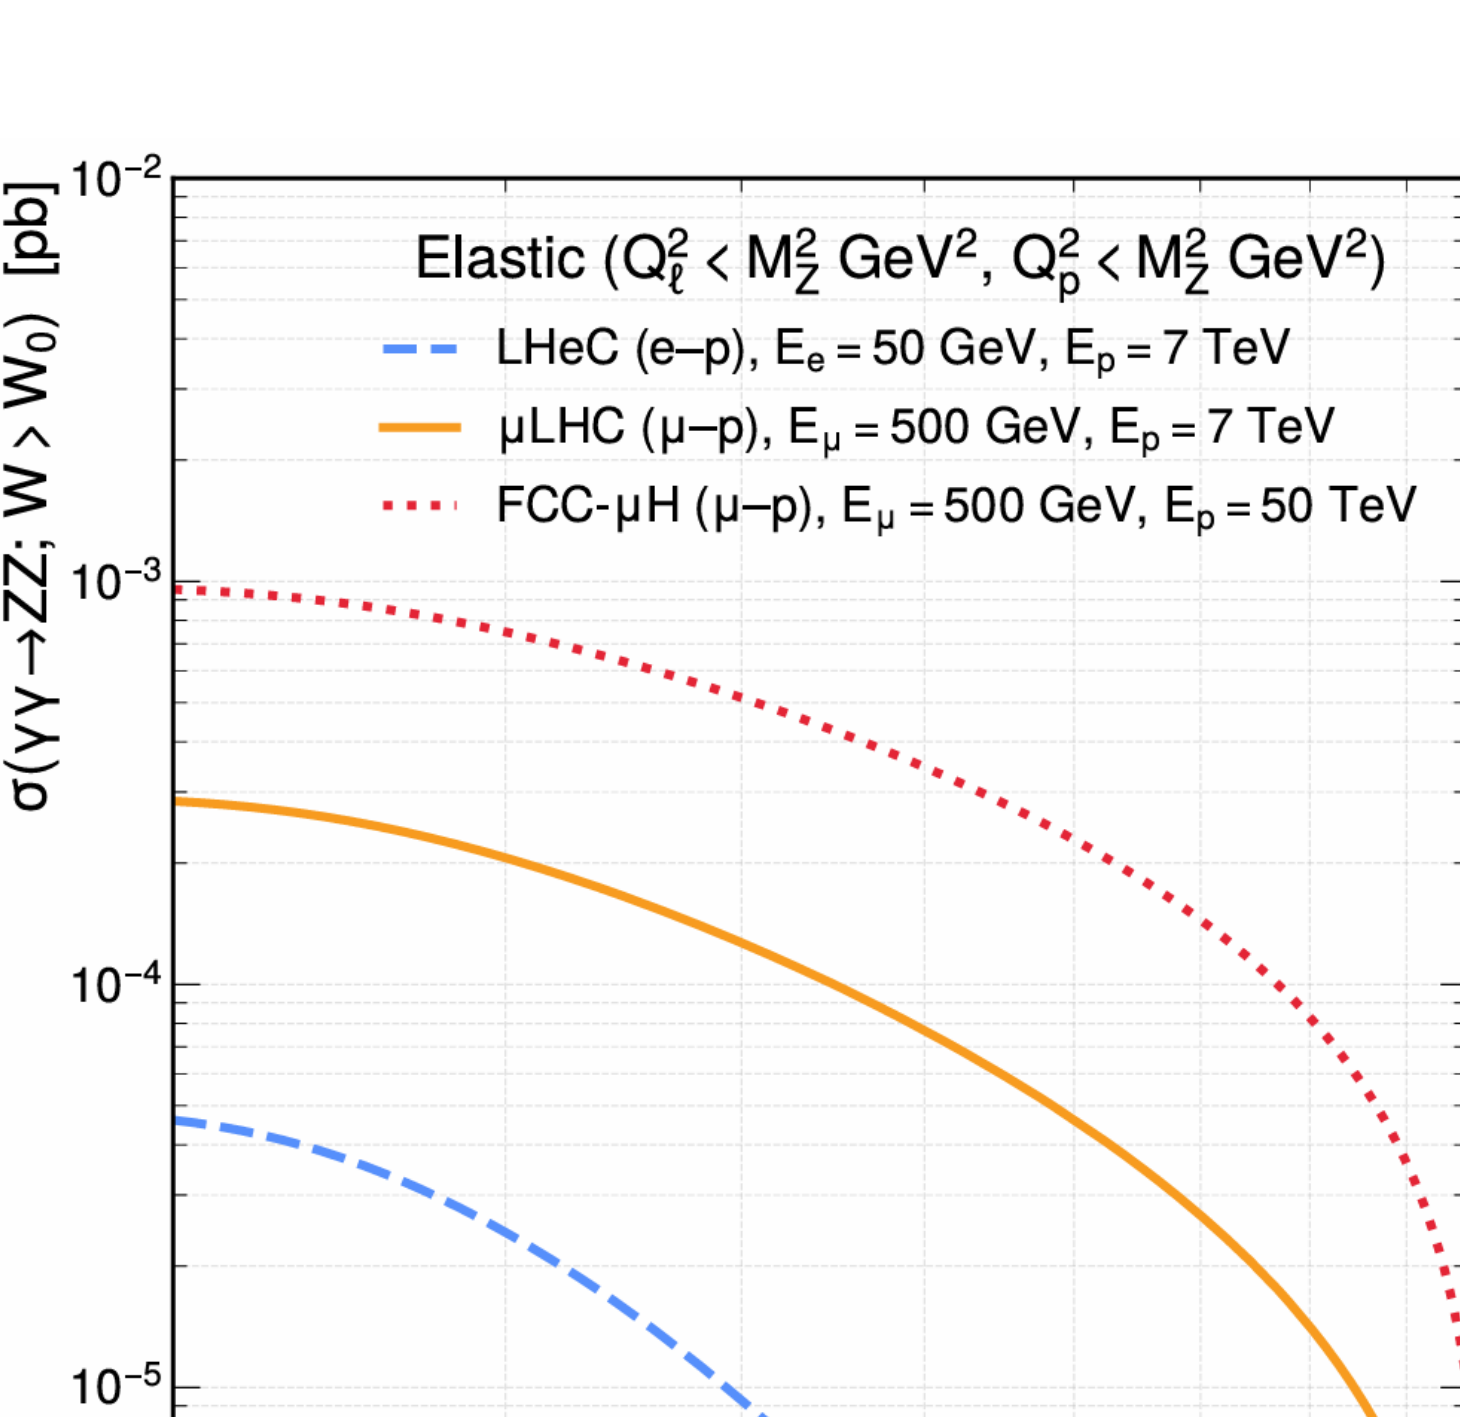
\includegraphics[width=0.68\linewidth]{zz_elastic_curve.png}
\end{column}
\begin{column}{0.40\textwidth}
\begin{itemize}\scriptsize
\item In the SM, $\gamma\gamma\to ZZ$ is absent at tree level and proceeds through loops.
\item The small SM rate makes the channel a clean window on anomalous neutral quartic interactions.
\item LH$\mu$C extends the accessible high-$M_{ZZ}$ regime.
\end{itemize}
\begin{alertblock}{Elastic benchmark}\scriptsize
\[
\sigma_{\rm el}^{\rm LHeC}\simeq0.046~\mathrm{fb}
\]
\[
\boxed{\sigma_{\rm el}^{\rm LH\mu C(3.7)}\simeq0.284~\mathrm{fb}}
\]
\end{alertblock}
\end{column}
\end{columns}
\sourceline{Existing HELP4CERN elastic $ZZ$ calculation; updated draft motivates the neutral-QGC study.}
\helplogo
\end{frame}

% --------------------------------------------------------------------------
% Slide 21 -- Source: updated draft_yy_lhec ZZ AQGC table
% --------------------------------------------------------------------------

\begin{frame}{Neutral quartic gauge couplings in $\gamma\gamma\to ZZ$}
\begin{columns}[T]
\begin{column}{0.56\textwidth}
\begin{block}{Rate model used in the updated study}\scriptsize
\[
\sigma_{\rm tot}\simeq\sigma_{\rm SM}^{\rm loop}+\sigma_{\rm AQGC}^{\rm tree}.
\]
\end{block}
\begin{alertblock}{LHeC tagged-elastic reference}\tiny
$\sigma_{\rm SM}=3.340\times10^{-5}$ pb; raw events assume 1 ab$^{-1}$ before $Z$ decays and detector effects.\par\smallskip
\centering
\begin{tabular}{cccc}
\toprule
$f_{M2}/\Lambda^4$ & $\sigma_{\rm AQGC}$ [pb] & events & enhancement\\
\midrule
0.1 & $1.17\times10^{-8}$ & 0.012 & 1.0004\\
1.0 & $1.17\times10^{-6}$ & 1.17 & 1.035\\
5.0 & $2.93\times10^{-5}$ & 29.3 & 1.88\\
\bottomrule
\end{tabular}
\end{alertblock}
\end{column}
\begin{column}{0.40\textwidth}
\begin{itemize}\scriptsize
\item SM is loop induced; the quoted AQGC contribution is tree level.
\item The table shows how an energy-growing neutral interaction can become competitive with a rare SM channel.
\item These are \textbf{LHeC reference numbers}, not LH$\mu$C projected limits; the harder LH$\mu$C spectrum motivates the direct extension.
\end{itemize}
\end{column}
\end{columns}
\sourceline{Updated draft\_yy\_lhec, neutral aQGC section.}
\helplogo
\end{frame}

% --------------------------------------------------------------------------
\section{Heavy and BSM final states}

% Slide 22 -- Adapted from existing gamma-gamma ttbar benchmark
% --------------------------------------------------------------------------

\begin{frame}{Heavy final states: $\gamma\gamma\to t\bar t$}
\begin{columns}[T]
\begin{column}{0.56\textwidth}
\centering
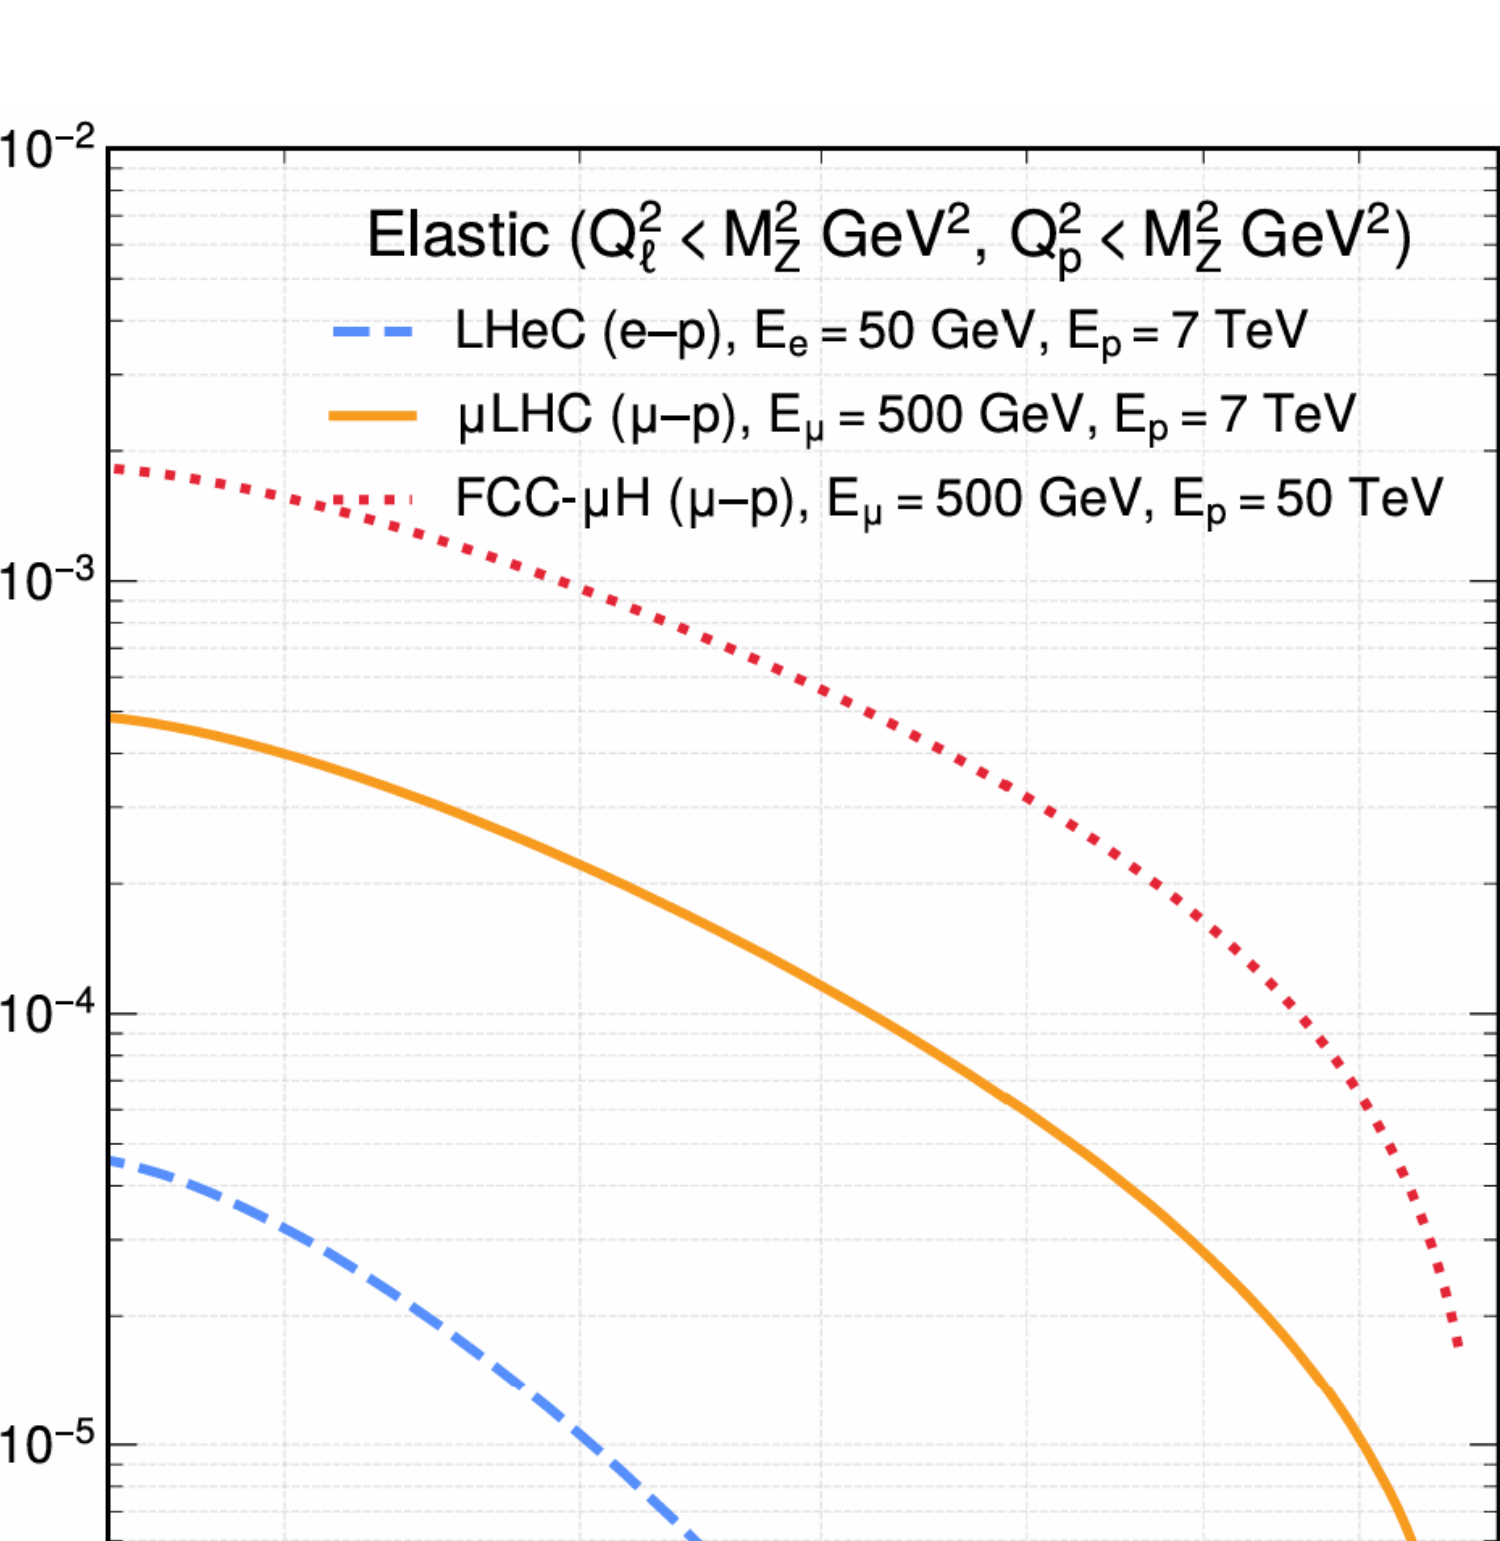
\includegraphics[width=0.68\linewidth]{ttbar_elastic_curve.png}
\end{column}
\begin{column}{0.40\textwidth}
\begin{alertblock}{Elastic benchmark}\scriptsize
\[
\sigma_{\rm el}^{\rm LHeC}\simeq0.046~\mathrm{fb}
\]
\[
\boxed{\sigma_{\rm el}^{\rm LH\mu C(3.7)}\simeq0.486~\mathrm{fb}}
\]
\end{alertblock}
\begin{itemize}\scriptsize
\item This is exclusive $\gamma\gamma\to t\bar t$ --- \textbf{not} the much larger $\gamma g\to t\bar t$ photoproduction channel.
\item The $2m_t$ threshold probes the hard end of the photon spectrum.
\item The channel accesses the top electromagnetic interaction and high-energy new physics.
\end{itemize}
\end{column}
\end{columns}
\sourceline{Existing HELP4CERN elastic $\gamma\gamma\to t\bar t$ calculation.}
\helplogo
\end{frame}

% --------------------------------------------------------------------------
% Slide 23 -- Source: yy_lhec SUSY section + updated compressed-SUSY discussion
% --------------------------------------------------------------------------

\begin{frame}{Beyond the Standard Model: charged-particle pair production in $\gamma\gamma$ collisions}
\begin{columns}[T]
\begin{column}{0.56\textwidth}
\centering
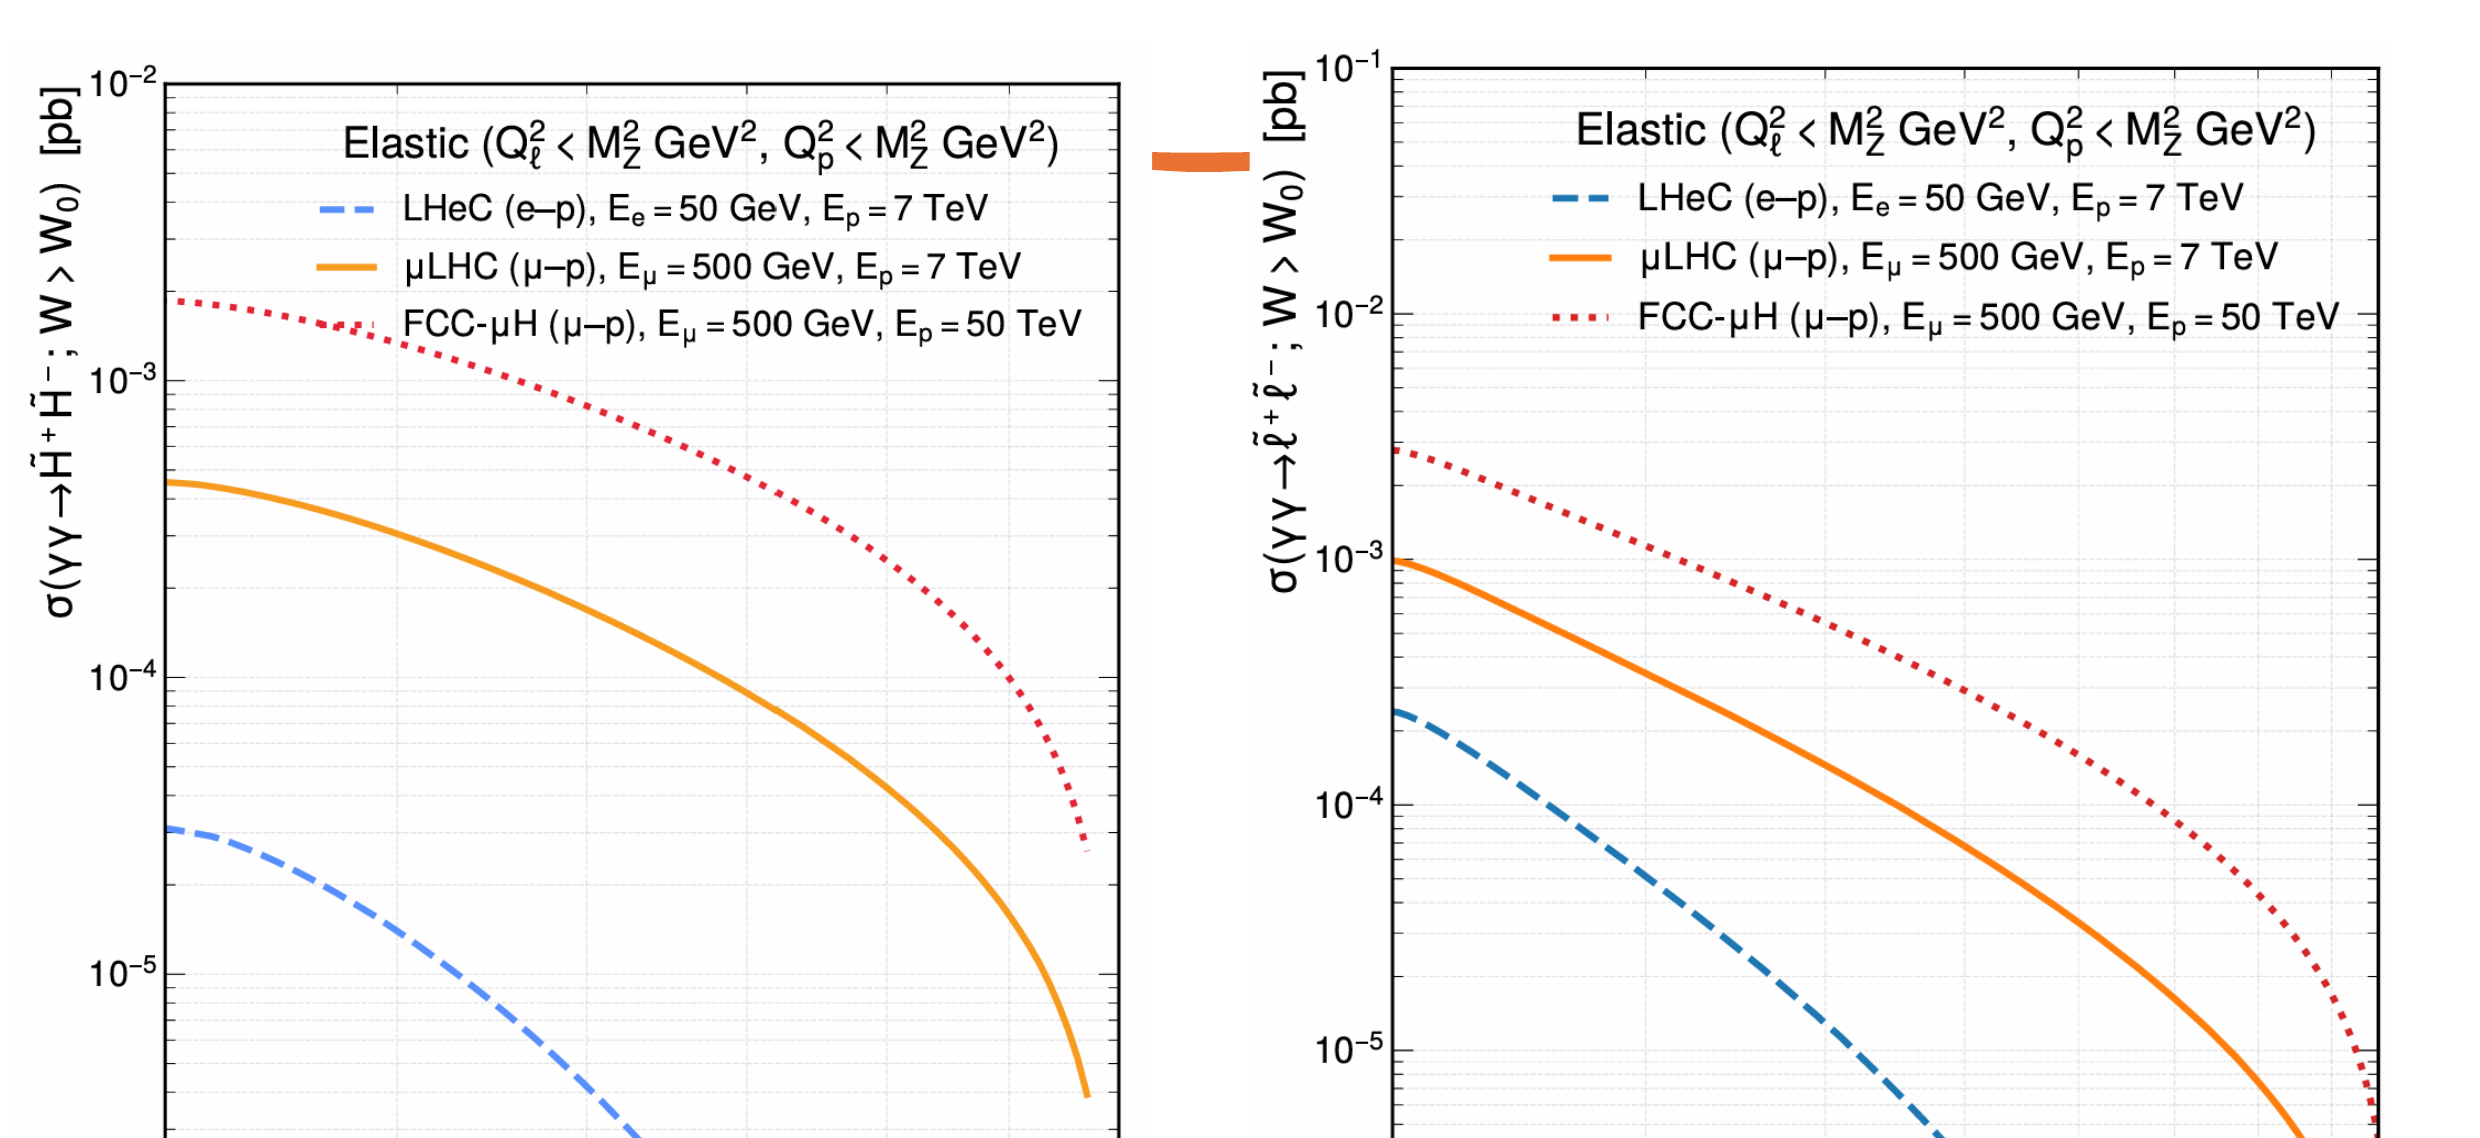
\includegraphics[width=0.80\linewidth]{susy_pair_curves.png}
{\tiny Illustrative 100 GeV scalar (slepton) and fermion (higgsino) reference curves.}
\end{column}
\begin{column}{0.41\textwidth}
\begin{itemize}\scriptsize
\item Representative channels:
\[
\gamma\gamma\to\tilde\ell^+\tilde\ell^-,\qquad
\gamma\gamma\to\tilde\chi^+\tilde\chi^-.
\]
\item Rates are governed mainly by electric charge and mass, complementary to strongly interacting searches.
\item Forward kinematic closure is attractive for compressed spectra with soft visible products and missing momentum.
\end{itemize}
\begin{alertblock}{Updated interpretation}\tiny
The draft notes that 100 GeV is now illustrative. Current constraints motivate roughly 300 GeV sleptons and 250--300 GeV higgsino benchmarks; LHeC rates near those thresholds are tiny, making a dedicated LH$\mu$C re-evaluation especially relevant.
\end{alertblock}
\end{column}
\end{columns}
\sourceline{yy\_lhec SUSY section + updated compressed-SUSY discussion in draft\_yy\_lhec.}
\helplogo
\end{frame}

% --------------------------------------------------------------------------
% Slide 24 -- Source: updated LbL section + Higgs section
% --------------------------------------------------------------------------

\begin{frame}{Light-by-light scattering, Higgs production, and other $\gamma\gamma$ opportunities}
\begin{columns}[T]
\begin{column}{0.58\textwidth}
\begin{block}{Mature calculation: $\gamma\gamma\to\gamma\gamma$}\scriptsize
SM light-by-light scattering is loop induced; all charged SM particles contribute to the box amplitude.
\end{block}
\centering
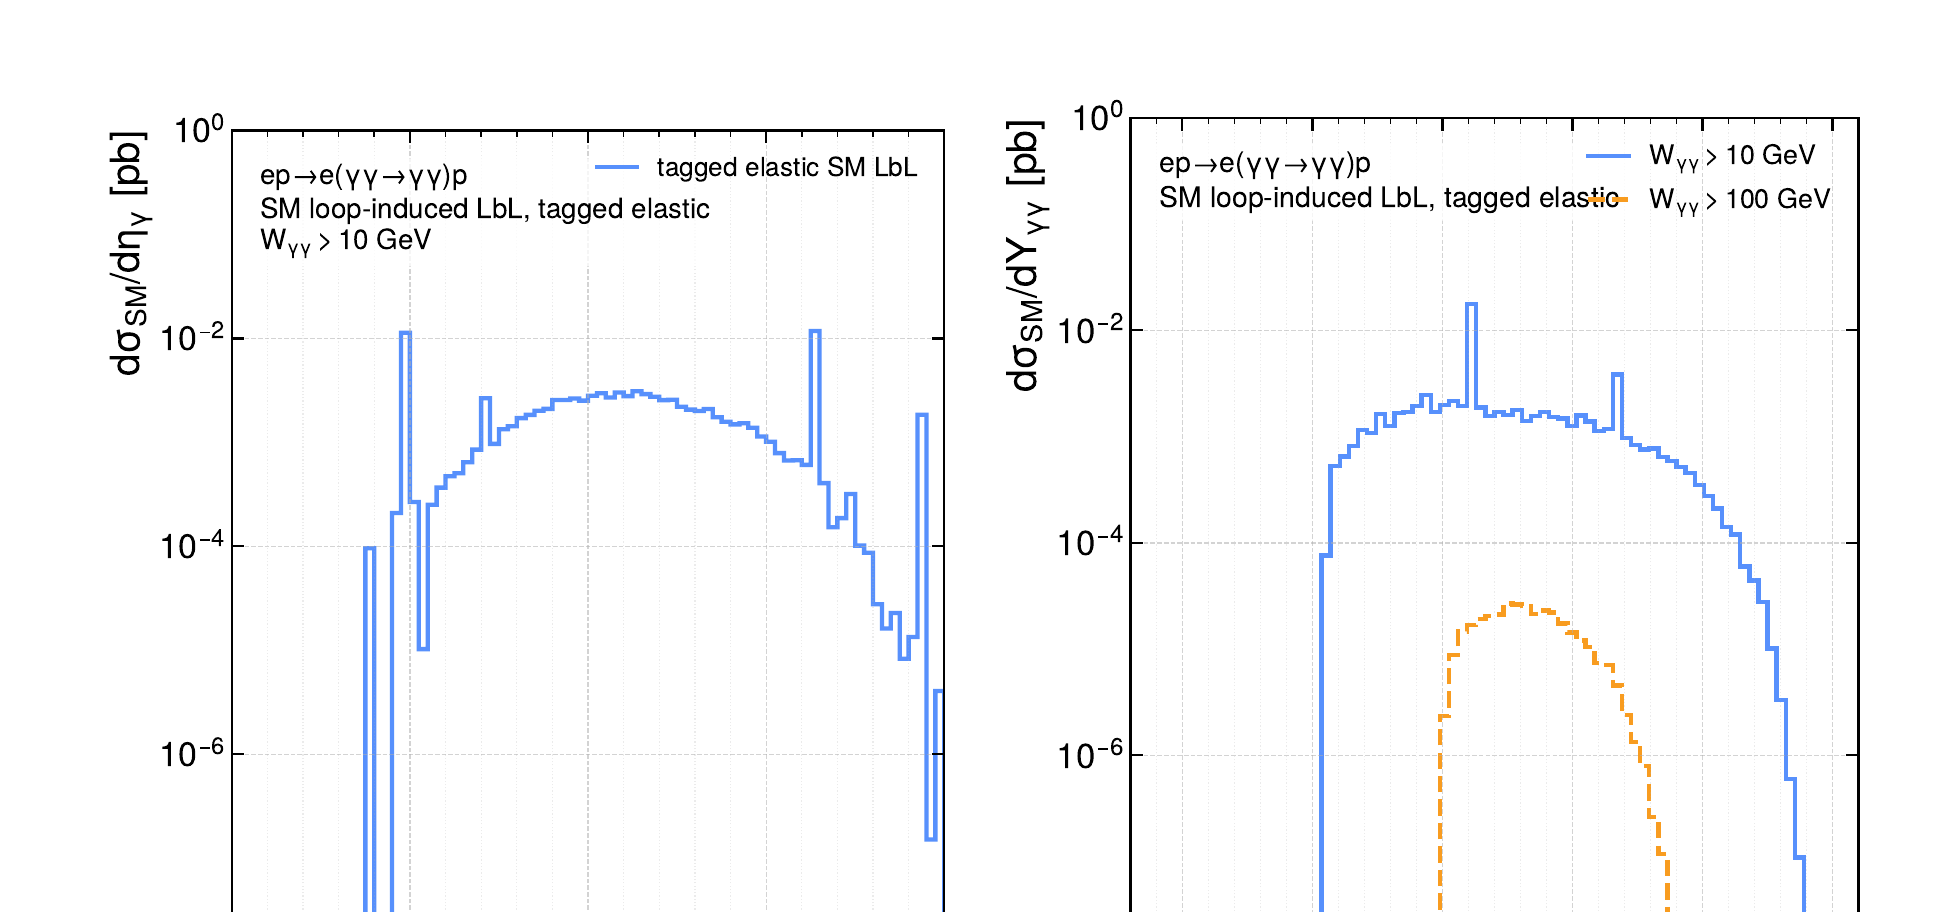
\includegraphics[width=0.80\linewidth]{lbl_eta_updated.png}
{\tiny Updated LHeC tagged-elastic SM pseudorapidity distributions.}
\end{column}
\begin{column}{0.39\textwidth}
\begin{alertblock}{Exploratory: $\gamma\gamma\to H$}\scriptsize
The Higgs channel is loop induced and rare, but it probes the effective $H\gamma\gamma$ interaction in an exceptionally clean initial state.
\end{alertblock}
\centering
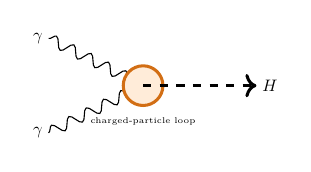
\begin{tikzpicture}[scale=0.60,transform shape]
\coordinate (a) at (-2,1);\coordinate (b) at (-2,-1);\coordinate (c) at (0,0);\coordinate (h) at (2.4,0);
\draw[decorate,decoration={snake,amplitude=2pt,segment length=7pt}] (a)--(c);
\draw[decorate,decoration={snake,amplitude=2pt,segment length=7pt}] (b)--(c);
\draw[fill=orange!15,draw=LHOrange,line width=1.1pt] (c) circle (0.42);
\draw[dashed,line width=1.1pt,->] (c)--(h);
\node[left] at (a) {$\gamma$};\node[left] at (b) {$\gamma$};\node[right] at (h) {$H$};
\node[font=\tiny] at (0,-0.75) {charged-particle loop};
\end{tikzpicture}
\begin{block}{LH$\mu$C opportunity}\scriptsize
The harder photon spectrum extends the high-mass LbL region and other loop-induced or resonant searches.
\end{block}
\end{column}
\end{columns}
\sourceline{Updated draft\_yy\_lhec LbL section; Higgs-via-$\gamma\gamma$ section in yy\_lhec / draft\_yy\_lhec.}
\helplogo
\end{frame}

% --------------------------------------------------------------------------
\section{Experimental opportunities and outlook}

% Slide 25 -- New experiment-facing summary
% --------------------------------------------------------------------------

\begin{frame}{What does two-photon physics require from the LH$\mu$C experiment?}
\begin{columns}[T]
\begin{column}{0.58\textwidth}
\begin{itemize}\scriptsize
\item \textbf{Wide central tracking and lepton acceptance}, including robust $\tau$ reconstruction.
\item \textbf{Efficient $W/Z/t$ reconstruction} for heavy $\gamma\gamma$ final states.
\item \textbf{Exclusivity and acoplanarity} observables with sensitivity to low extra activity.
\item \textbf{Missing-momentum performance} for neutrinos and compressed BSM signatures.
\item \textbf{Scattered-muon measurement} to constrain the lepton-side photon kinematics.
\item \textbf{Forward proton tagging where feasible}, together with control of proton dissociation.
\item Exploit the defining advantage: the \textbf{clean, low-pile-up $\mu p$ environment}.
\end{itemize}
\begin{alertblock}{Physics--detector connection}\scriptsize
The $\gamma\gamma$ programme links central reconstruction, lepton tagging and near-beam instrumentation directly to the usable photon luminosity and kinematic closure.
\end{alertblock}
\end{column}
\begin{column}{0.38\textwidth}
\placeholdergraphic{Suggested figure: LH$\mu$C interaction-region schematic with central detector, scattered-muon acceptance and a near-beam proton tag.}{3.05cm}
\end{column}
\end{columns}
\helplogo
\end{frame}

% --------------------------------------------------------------------------
% Slide 26 -- Final summary, no separate 27th thank-you slide
% --------------------------------------------------------------------------

\begin{frame}{Summary and outlook}
\begin{columns}[T]
\begin{column}{0.75\textwidth}
\begin{itemize}\small
\item LH$\mu$C turns $\mu p$ collisions into a \textbf{high-energy $\gamma\gamma$ laboratory} with a substantially harder photon spectrum than the LHeC benchmark.
\item EPA and $S_{\gamma\gamma}$ connect parent $\mu p$ luminosity transparently to elastic and proton-dissociative two-photon subprocesses.
\item $\tau^+\tau^-$ and $W^+W^-$ provide high-statistics precision/EFT channels; sensitivity lives in their hard invariant-mass tails.
\item Loop-induced $ZZ$, exclusive $t\bar t$, light-by-light scattering, $H$, and charged BSM pairs extend the programme to rare quantum processes and heavy thresholds.
\end{itemize}
\vspace{0.3em}
{\small\color{LHRed}\textbf{Bottom line: high-energy $\gamma\gamma$ physics is one of the distinctive physics opportunities of LH$\mu$C.}}
\end{column}
\begin{column}{0.21\textwidth}
\centering
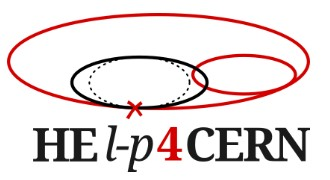
\includegraphics[width=0.88\linewidth]{HELP4CERN.jpg}
\vspace{0.7em}

{\Large\bfseries Thank you!}
\vspace{0.5em}

{\tiny Hamzeh Khanpour\\AGH University of Krakow\\\texttt{hamzeh.khanpour@cern.ch}}
\end{column}
\end{columns}
\end{frame}

\end{document}
